\documentclass[11pt]{article}
	
	%%%%%%%%%%%%%%%%%%%%%%%%%%%%%%%%%%%%%%%%%%%%%%%%%%%%%%%%%%%%%%%%%%%%%%
	%\pdfminorversion=4
	% NOTE: To produce blinded version, replace "0" with "1" below.
	\newcommand{\blind}{0}
	
	\AddToHook{cmd/section/before}{\clearpage} % all sections in new page
	
	%%%%%%% IISE Transactions margin specifications %%%%%%%%%%%%%%%%%%%
	% DON'T change margins - should be 1 inch all around.
	\addtolength{\oddsidemargin}{-.5in}%
	\addtolength{\evensidemargin}{-.5in}%
	\addtolength{\textwidth}{1in}%
	\addtolength{\textheight}{1.3in}%
	\addtolength{\topmargin}{-.8in}%
    \makeatletter
    \renewcommand\section{\@startsection {section}{1}{\z@}%
                                       {-3.5ex \@plus -1ex \@minus -.2ex}%
                                       {2.3ex \@plus.2ex}%
                                       {\normalfont\fontfamily{phv}\fontsize{16}{19}\bfseries}}
    \renewcommand\subsection{\@startsection{subsection}{2}{\z@}%
                                         {-3.25ex\@plus -1ex \@minus -.2ex}%
                                         {1.5ex \@plus .2ex}%
                                         {\normalfont\fontfamily{phv}\fontsize{14}{17}\bfseries}}
    \renewcommand\subsubsection{\@startsection{subsubsection}{3}{\z@}%
                                        {-3.25ex\@plus -1ex \@minus -.2ex}%
                                         {1.5ex \@plus .2ex}%
                                         {\normalfont\normalsize\fontfamily{phv}\fontsize{14}{17}\selectfont}}
    \makeatother
    %%%%%%%%%%%%%%%%%%%%%%%%%%%%%%%%%%%%%%%%%%%%%%%%%%%%%%%%%%%%%%%%%%%%%%%%%
	
	%%%%% IISE Transactions package list %%%%%%%%%%%%%%%%%%%%%%%%%%%%%%%%%%%%%%
	\usepackage{enumerate}
	\usepackage{xcolor}
	\usepackage{graphicx}	% rotate row
	\usepackage{soul}		% highlight
	\usepackage{url} 		% not crucial - just used below for the URL
	\usepackage{bytefield} 	% network protocol
	\usepackage{hyperref} 	% go to labels on click
	\usepackage{chngcntr}	% count figures/tables with sections
	\usepackage{footnote}	% notes inside tables
	\usepackage{float}		% place figures exactly there
	\usepackage{longtable}	% tables that are more than one page size
	\usepackage{subfloat}	% subfigures
	\usepackage{pifont}
	\usepackage[natbibapa]{apacite}	% bibliography
	\usepackage[acronym,section=subsection]{glossaries}
	%%%%%%%%%%%%%%%%%%%%%%%%%%%%%%%%%%%%%%%%%%%%%%%%%%%%%%%%%%%%%%%%%%%%%%%
	
	
	% diagram imports
	\usepackage{tikz}
	\usepackage{drawstack}
	\usepackage{adjustbox}
	\usetikzlibrary{shapes.geometric, arrows, positioning, calc}
	
	\tikzstyle{process} = [rectangle, minimum width=3cm, minimum height=1cm, align=center, draw=black, fill=orange!30]
	\tikzstyle{arrow} = [thick,->,>=stealth]
	\tikzstyle{generalization} = [thick, ->, -triangle 90, fill=white] % TODO why not working
	
	
	% centered bytefield
	\newenvironment{cbytefield}
		{\begin{center}\begin{bytefield}}
		{\end{bytefield}\end{center}}
	
	% rename titles
	\renewcommand{\listfigurename}{Figures}
	\renewcommand{\listtablename}{Tables}
	
	% allow footnotes inside tabular
	\makesavenoteenv{tabular}
	\makesavenoteenv{table}
	\makesavenoteenv{figure}
	
	% count figures/tables with sections
	\counterwithin{table}{section}
	\counterwithin{figure}{section}
	
	% check/cross mark
	\newcommand{\cmark}{\ding{51}}%
	\newcommand{\xmark}{\ding{55}}%
	
	% TODOs
	\newcommand\myworries[1]{\sethlcolor{red}\hl{#1}}
	
	% place here
	\restylefloat{figure}
	\restylefloat{table}
	
	% acronyms
	\makeglossaries
	\loadglsentries{glossaries}
	

	
	%%%%% Author package list and commands %%%%%%%%%%%%%%%%%%%%%%%%%%%%%%%%%%%%%%%%%%%%%
	%%%%% Here are some examples %%%%%%%%%%%%%%
	%	\usepackage{amsfonts, amsthm, latexsym, amssymb}
	%	\usepackage{lineno}
	%	\newcommand{\mb}{\mathbf}
	%%%%%%%%%%%%%%%%%%%%%%%%%%%%%%%%%%%%%%%%%%%%%%%%%%%%%%%%%%%%%%%%%%%%%%%%%%%%%%
	
	\begin{document}
		
			%%%%%%%%%%%%%%%%%%%%%%%%%%%%%%%%%%%%%%%%%%%%%%%%%%%%%%%%%%%%%%%%%%%%%%%%%%%%%%
		\def\spacingset#1{\renewcommand{\baselinestretch}%
			{#1}\small\normalsize} \spacingset{1}
		%%%%%%%%%%%%%%%%%%%%%%%%%%%%%%%%%%%%%%%%%%%%%%%%%%%%%%%%%%%%%%%%%%%%%%%%%%%%%%
		
		\title{\bf WatchWolf API Definition}
		\author{WatchWolf Contributors}
		\date{}
		\maketitle
		\bigskip
			
	\noindent%
	{\it Keywords:} \emph{WatchWolf}; Minecraft plugin testing; Integration testing environment.

	%\newpage
	\spacingset{1.5} % DON'T change the spacing!

\maketitle
\tableofcontents

\listoffigures

\listoftables

\section{Documentation conventions}
%\myworries{...}

% Acronyms
\printglossary[numberedsection,type=\acronymtype]

% Glossary
\printglossary[numberedsection]

\section{WatchWolf Introduction} \label{s:intro}
WatchWolf is an integration testing environment for Minecraft plugins. It will validate that your plugin works using multiple real \acrshort{mc} servers of different types and versions.

In order to achieve that, WatchWolf splits into 4 different programs, each one with one responsibility:
\begin{enumerate}
	\item WatchWolf Tester
	
		WatchWolf Tester if the entry point to the WatchWolf environment.\footnote{The WatchWolf environment is the combination of all the WatchWolf parts: Tester, Servers Manager, Server, Clients Manager and Client.} It will orchestrate all the setup/stop process and run the user tests.
	
	\item WatchWolf Servers Manager
	
		WatchWolf Servers Manager provides \acrshort{mc} servers on-demand. It will start them and, after they have been closed, free the allocated resources.
	
	\item WatchWolf Server
	
		WatchWolf Server is the actual \acrshort{mc} server. It will contain the plugin to test and run the commands sent by WatchWolf Tester.
	
	\item WatchWolf Clients Manager
	
		WatchWolf Clients Manager is the same as WatchWolf Servers Manager, but for clients. It will starts clients on-demand and connect them to the servers allocated by WatchWolf.
	
	\item WatchWolf Client
	
		WatchWolf Client is a \acrshort{mc} client, with the ability to connect to one server and interact with it.
\end{enumerate}

You can see with more detail how the different programs relations on the \hyperref[fig:diagram]{Figure \ref{fig:diagram}, Diagram representing WatchWolf's most important actuators}.

\begin{figure}[H]
	\centering
	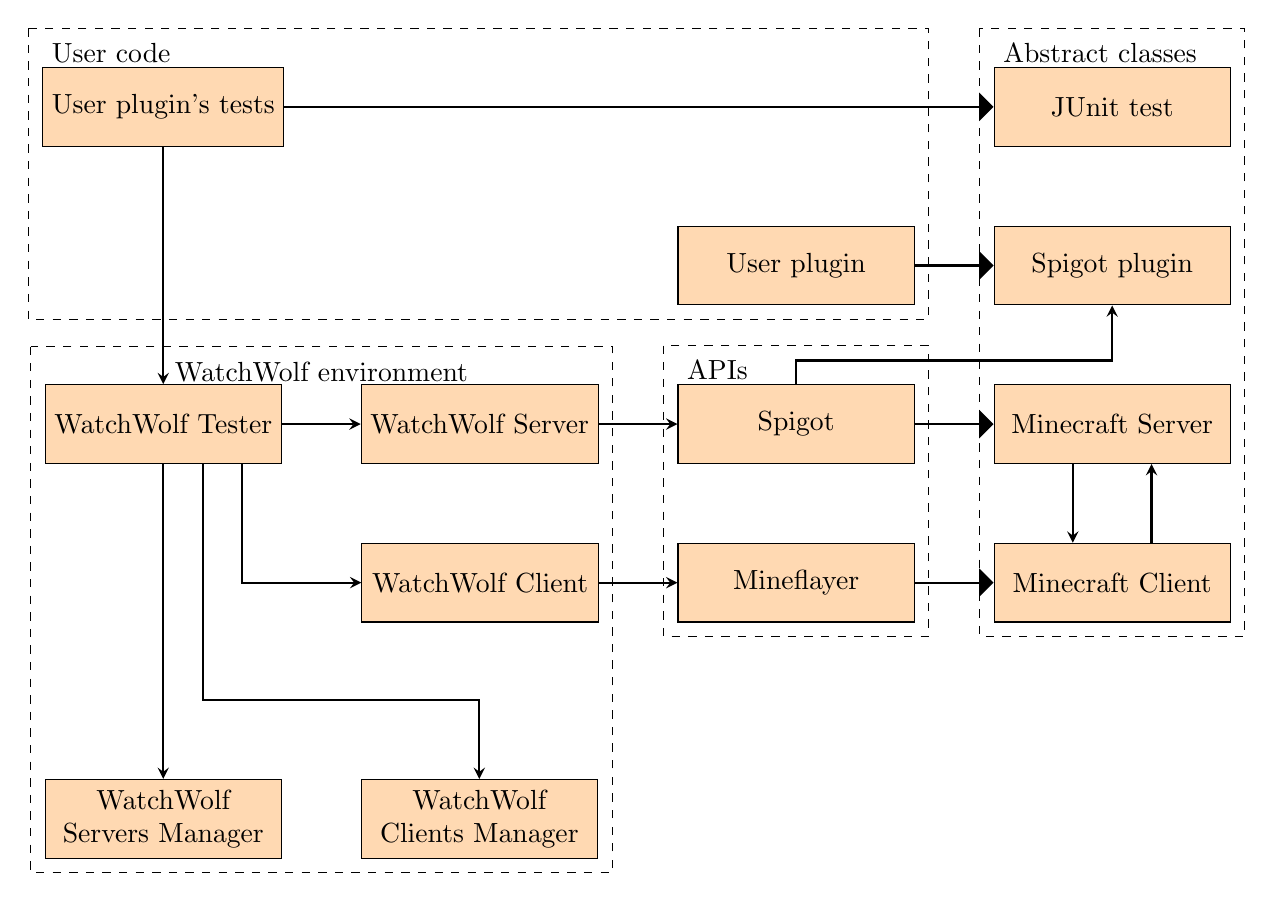
\begin{tikzpicture}[node distance=1cm]
	% nodes
	\node (plugin) [process] {User plugin};
	
	\node (spigot) [process, below=of plugin] {Spigot};
	
	\node (server) [process, left=of spigot] {WatchWolf Server};
	
	\node (tester) [process, left=of server] {WatchWolf Tester};
	
	\node(mc-server) [process, right=of spigot] {Minecraft Server};
	
	\node(spigot-plugin) [process, above=of mc-server] {Spigot plugin}; % implicit right=of plugin
	
	\node(junit) [process, above=of spigot-plugin] {JUnit test};
	
	\node (plugin-test) at (tester |- junit) [process] {User plugin's tests};
	
	\node (mc-client) [process, below=of mc-server] {Minecraft Client};
	
	\node (mineflayer) [process, left=of mc-client] {Mineflayer};
	
	\node (client) [process, left=of mineflayer] {WatchWolf Client};
	
	\node (servers-manager) [process, below=of tester, yshift=-3cm] {
		WatchWolf\\
		Servers Manager
	};
	
	\node (clients-manager) [process, right=of servers-manager] {
		WatchWolf\\
		Clients Manager
	};
	
	% wrappers
	\node(watchwolf-wrapper-text) [above=12pt of $(tester)!0.5!(server)$] {WatchWolf environment};
	\draw[dashed] ([xshift=-5pt,yshift=2pt] tester.west |- watchwolf-wrapper-text.north) rectangle ([xshift=5pt,yshift=-5pt] clients-manager.south -| client.east);
	
	\node(user-wrapper-text) [right=0 of plugin-test.north west, yshift=5pt] {User code};
	\draw[dashed] ([xshift=-5pt,yshift=2pt] user-wrapper-text.north west) rectangle ([xshift=5pt,yshift=-5pt] plugin.south east);
	
	\node(abstract-wrapper-text) [right=0 of junit.north west, yshift=5pt] {Abstract classes};
	\draw[dashed] ([xshift=-5pt,yshift=2pt] abstract-wrapper-text.north west) rectangle ([xshift=5pt,yshift=-5pt] mc-client.south east);
	
	\node(abstract-impl-wrapper-text) [right=0 of spigot.north west, yshift=5pt] {APIs};
	\draw[dashed] ([xshift=-5pt,yshift=2pt] abstract-impl-wrapper-text.north west) rectangle ([xshift=5pt,yshift=-5pt] mineflayer.south east);
	
	
	% arrows
	\draw [arrow] (plugin-test) -- (tester);
	\draw [arrow] (spigot.north) -- ++(0,0.3) -| (spigot-plugin);
	\draw [arrow] (tester) -- (server);
	\draw [arrow] ([xshift=1cm] tester.south) |- (client.west);
	\draw [arrow] (tester) -- (servers-manager);
	\draw [arrow] ([xshift=0.5cm] tester.south) |- ([yshift=1cm] clients-manager.north) -- (clients-manager);
	\draw [arrow] (server) -- (spigot);
	\draw [arrow] (client) -- (mineflayer);
	\draw [generalization] (mineflayer) -- (mc-client);
	\draw [generalization] (spigot) -- (mc-server);
	\draw [generalization] (plugin) -- (spigot-plugin);
	\draw [generalization] (plugin-test) -- (junit);
	\draw [arrow] ([xshift=-0.5cm] mc-server.south) -- ([xshift=-0.5cm] mc-client.north);
	\draw [arrow] ([xshift=0.5cm] mc-client.north) -- ([xshift=0.5cm] mc-server.south);
\end{tikzpicture}
	
	\caption{Diagram representing WatchWolf's most important actuators}
	\label{fig:diagram}
\end{figure}

\section{API Introduction}
In order to interact with the different WatchWolf modules, you'll have to follow the WatchWolf API: a series of supported operations in one program. All the packets sent \& received will follow the structure shown in \hyperref[fig:packet-structure]{Figure \ref{fig:packet-structure}, Packet structure}.

\begin{figure}[H]
	\centering
	\begin{bytefield}{32}
		\bitheader{0,2,3,4,15,16,31} \\
		\bitbox{3}{\hyperref[s:dst]{DST}} & \bitbox{1}{\hyperref[s:response]{r}} & \bitbox{12}{\hyperref[s:operation]{operation}} & \bitbox[lrt]{16}{} \\
		\wordbox[lr]{1}{\hyperref[s:args]{arguments}} \\
		\skippedwords \\
		\wordbox[lrb]{1}{}
	\end{bytefield}
	\caption{Packet structure}
	\label{fig:packet-structure}
\end{figure}

\subsection{Destiny} \label{s:dst}
The first argument (\textit{DST}) will be the destiny of that packet. This will specify one of the 4 modules connected to WatchWolf Tester (for more information refer to \hyperref[s:intro]{Section \ref{s:intro}, WatchWolf Introduction}). Note that WatchWolf Tester itself is not present, as it will be indicated with the \hyperref[s:response]{Response} bit at 1. You can see the different \textit{DST} values for each module om the \hyperref[fig:dst]{Figure \ref{fig:dst}, DST bits meaning}.

\begin{table}[H]
	\centering
	\begin{tabular}{ |c|c|c|c| }
		\hline
		DST[2] & DST[1] & DST[0] & Destination \\
		\hline
		0 & 0 & 0 & ServerManagerPetition \\
		0 & 0 & 1 & ServerPetition \\
		0 & 1 & 0 & ClientsManagerPetition \\
		0 & 1 & 1 & ClientPetition \\
		\hline
		1 & X & X & \textit{Reserved} \\
		\hline
	\end{tabular}
	\caption{DST bits meaning}
	\label{fig:dst}
\end{table}

\subsection{Response} \label{s:response}
Some of the petitions have return objects. Those petitions will return to the sender (TesterConnector) with the same code, but with a '1' on the Response parameter. In that case, the parameter \hyperref[s:dst]{Destiny} now means 'Origin'.

Some petitions have \gls{async} "returns" (e.g. \hyperref[s:error-notification]{Error notification}). Those will be sent directly marked as responses (Response bit at '1').

\subsection{Operation} \label{s:operation}
The Operation parameter specifies the desired request. Those change according to the \hyperref[s:dst]{Destiny}, so they will be discussed in more detail in their respective sections.

The only exception is the all-zeroes operation (0b000000000000) which represents a \gls{NOP} request. That way, if you need to perform a long test, you won't be kicked by inactivity\footnote{This is a safety mechanism to avoid blocking a server to the same user forever. \myworries{Besides being defined by the API it hasn't been implemented yet, and won't be until WatchWolf offers public servers.}} if you send this request every few minutes.

\subsection{Arguments} \label{s:args}
The Arguments parameter specifies the arguments (if any) to the \textit{\hyperref[s:operation]{Operation}} request. Those change according to the \hyperref[s:dst]{Destiny}, so the amount of arguments, and their types and order will be discussed in more detail in their respective sections.

Now there will be discussed the most common data types, so they will be independent of any programming language.

\subsubsection{Character}\label{type:char}
Characters are sent as a 1-byte integer, representing its ASCII \myworries{ref?} value.

\subsubsection{Boolean}\label{type:bool}
Booleans are 1-bit element that represents \textit{true} (0b1), or \textit{false} (0b0).

For alignment \myworries{define?} reasons, booleans will be sent as 1-byte element. To avoid misunderstandings, let's define \textit{false} as 0x00, and \textit{true} as '\textit{not \myworries{define?} false}'. That way, this two packets are valid \textit{true} elements:

\begin{figure}[H]
	\centering
	\begin{bytefield}{8}
		\bitheader{0,7} \\
		\bitbox{8}{0x01}
	\end{bytefield}
	\caption{True packet with the \glslink{LSB}{LSB} at 1}
\end{figure}

\begin{figure}[H]
	\centering
	\begin{bytefield}{8}
		\bitheader{0,7} \\
		\bitbox{8}{0xFF}
	\end{bytefield}
	\caption{True packet with all bits at 1}
\end{figure}

\subsubsection{Double}\label{type:double}
Doubles are 8-bytes floating-point numbers. They are represented following the \gls{IEEE-754}\footnote{This standard should be used by C, Java and Python. \myworries{cite?}}.

\subsubsection{String}\label{type:str}
Strings are \hyperref[type:array]{arrays} of \hyperref[type:char]{characters}. Refer to the respective subsections for more information.

\subsubsection{Array}\label{type:array}
Arrays are a set of \textit{n} elements of the same type.

The structure is a 2-byte \myworries{first (0..7) MSB, then (8..15) LSB} integer (representing the number of elements, \textit{n}), followed by \textit{n} elements of the same type. As a note here, by representing the size with a 2-byte integer the maximum number of elements per array is 65,535.

\begin{figure}[H]
	\centering
	\begin{bytefield}{32}
		\bitheader{0,15,16,23,24,31} \\
		\bitbox{16}{size} & \bitbox{8}{char[0]} & \bitbox{8}{char[1]} \\
		\wordbox[ltr]{1}{...} \\
		\skippedwords \\
		\wordbox[lrb]{1}{} \\
		\bitbox{8}{char[n-4]} & \bitbox{8}{char[n-3]} & \bitbox{8}{char[n-2]} & \bitbox{8}{char[n-1]}
	\end{bytefield}
	\caption{Structure of a \hyperref[type:str]{String}}
\end{figure}

Arrays can be \glslink{multidimensional-array}{multidimensional}, holding \textit{n} arrays of the same type. It's worth mentioning that they don't have to be arrays of the same length, as can be seen in Figure \ref{fig:multidimensional-array-example}, Example of a string array.
\begin{figure}[H]
	\centering
	\begin{bytefield}{32}
		\bitheader{0,15,16,23,24,31} \\
		\bitbox{16}{2 [number of arrays]} & \bitbox{16}{5 [str[0]'s length]} \\
		\bitbox{8}{h} & \bitbox{8}{e} & \bitbox{8}{l} & \bitbox{8}{l} \\
		\bitbox{8}{o} & \bitbox{16}{6 [str[1]'s length]} & \bitbox{8}{w} \\
		\bitbox{8}{o} & \bitbox{8}{r} & \bitbox{8}{l} & \bitbox{8}{d} \\
		\bitbox{8}{!} & \bitbox{24}[bgcolor=lightgray]{next type}
	\end{bytefield}
	\caption{Example of a string array}
	\label{fig:multidimensional-array-example}
\end{figure}

\subsubsection{File}\label{type:file}
Similar to the \hyperref[type:array]{Array}, a File is a name (\hyperref[type:str]{String}), followed by a group of bytes.

The problem here is that if we stick with the \hyperref[type:array]{Array} structure, the maximum size of a file will be around 8kB. To solve this, the File structure implements some kind of 'extended array', that extends the 'size' parameter to 32 bits. That way, the file size restriction by protocol definition\footnote{Besides defining here what's allowed, remember that this packet will be inside a TCP payload \myworries{definition?}. This means that the maximum file size will be probably redefined by the machine's TCP firewalls.} is 4GB.

\begin{figure}[H]
	\centering
	\begin{bytefield}{32}
		\bitheader{0,31} \\
		\wordbox[ltr]{1}{\hyperref[type:str]{file name}} \\
		\skippedwords \\
		\wordbox[lrb]{1}{} \\
		\wordbox[ltr]{1}{\hyperref[type:str]{file path\footnotemark}} \\
		\skippedwords \\
		\wordbox[lrb]{1}{} \\
		\bitbox{32}{file number of bytes} \\
		\wordbox[ltr]{1}{file contents} \\
		\skippedwords \\
		\wordbox[lrb]{1}{}
	\end{bytefield}
	\caption{File structure}
\end{figure}

% File structure's file path footnote
\footnotetext{The path must be relative, and you can't go outside the Server directory (using '../'). Both '' and './' means the root of the Server directory. \myworries{adding '' compatilibity}}

\subsubsection{Server type}\label{type:server-type}
The Server type specifies the Minecraft server.

As a standard, we only support Spigot (\cite{spigot-mc}) and Paper (\cite{paper-mc}), but for scalability reasons this parameter is a \hyperref[type:str]{String} specifying the server type.

\subsubsection{Position}\label{type:position}
\myworries{...}

\begin{figure}[H]
	\centering
	\begin{bytefield}{32}
		\bitheader{0,31} \\
		\wordbox[ltr]{1}{\hyperref[type:str]{world name}} \\
		\skippedwords \\
		\wordbox[lrb]{1}{} \\
		\wordbox[ltr]{1}{\hyperref[type:double]{x}} \\
		\wordbox[lrb]{1}{} \\
		\wordbox[ltr]{1}{\hyperref[type:double]{y}} \\
		\wordbox[lrb]{1}{} \\
		\wordbox[ltr]{1}{\hyperref[type:double]{z}} \\
		\wordbox[lrb]{1}{}
	\end{bytefield}
	\caption{Position structure}
\end{figure}

\subsubsection{Block}\label{type:block}
\myworries{... 56 bytes}



\begin{figure}[H]
	\centering
	\begin{bytefield}[bitwidth=2.5em]{16}
		\bitheader{0,7,8,9,10,11,12,13,14,15} \\
		\bitbox{15}{enum value} & \bitbox{1}[bgcolor=lightgray]{0} \\
		\bitbox{8}{\hyperref[spigot-types:age]{age}} &
		\bitbox{6}{\hyperref[spigot-types:direction]{direction}} & \bitbox{2}{\hyperref[spigot-types:axis]{axis}} \\
		
		\bitbox[lr]{8}[bgcolor=lightgray]{} &
		\bitbox{3}{\hyperref[spigot-types:groups]{group\_count}} & \bitbox{2}{\hyperref[spigot-types:delay]{delay}} &
		\bitbox{1}{\hyperref[spigot-types:eye]{eye}} & \bitbox{1}{\hyperref[spigot-types:hinge]{hinge}} &
		\bitbox{1}{\hyperref[spigot-types:open]{open}} \\
		\bitbox{8}{\hyperref[spigot-types:stages]{stage}} & 
		\bitbox{4}{\hyperref[spigot-types:parts]{part}} & \bitbox{4}{\hyperref[spigot-types:rotation]{rotation}} \\
		\bitbox{8}{\hyperref[spigot-types:note]{note}} &
		\bitbox{4}{\hyperref[spigot-types:mode]{mode}} & \bitbox{2}{\hyperref[spigot-types:leaves]{leaves}} & \bitbox{1}{\hyperref[spigot-types:lit]{lit}} & \bitbox{1}{\hyperref[spigot-types:locked]{locked}} \\
		\bitbox[lrt]{8}[bgcolor=lightgray]{} &
			\bitbox{1}{\hyperref[spigot-types:conditional]{cond}} & \bitbox{1}{\hyperref[spigot-types:inverted]{inv}} &
		\bitbox{1}{\hyperref[spigot-types:powered]{pow}} &
		\bitbox[lrt]{5}[bgcolor=lightgray]{} \\
		\bitbox[lr]{16}[bgcolor=lightgray]{} \\
		\bitbox[lr]{16}[bgcolor=lightgray]{reserved} \\
		\bitbox[lr]{16}[bgcolor=lightgray]{} \\
		\bitbox[lr]{16}[bgcolor=lightgray]{} \\
		\bitbox[lr]{16}[bgcolor=lightgray]{} \\
		\bitbox[lr]{16}[bgcolor=lightgray]{} \\
		\bitbox[lr]{16}[bgcolor=lightgray]{} \\
		\bitbox[lr]{16}[bgcolor=lightgray]{} \\
		\bitbox[lr]{16}[bgcolor=lightgray]{} \\
		\bitbox[lr]{16}[bgcolor=lightgray]{} \\
		\bitbox[lr]{16}[bgcolor=lightgray]{} \\
		\bitbox[lr]{16}[bgcolor=lightgray]{} \\
		\bitbox[lr]{16}[bgcolor=lightgray]{} \\
		\bitbox[lr]{16}[bgcolor=lightgray]{} \\
		\bitbox[lr]{16}[bgcolor=lightgray]{} \\
		\bitbox[lr]{16}[bgcolor=lightgray]{} \\
		\bitbox[lr]{16}[bgcolor=lightgray]{} \\
		\bitbox[lr]{16}[bgcolor=lightgray]{} \\
		\bitbox[lr]{16}[bgcolor=lightgray]{} \\
		\bitbox[lr]{16}[bgcolor=lightgray]{} \\
		\bitbox[lr]{16}[bgcolor=lightgray]{} \\
		\bitbox[lrb]{16}[bgcolor=lightgray]{} \\
	\end{bytefield}
	\caption{Structure of a \hyperref[type:block]{Block}}
\end{figure}

%\begin{figure}[H]
%	\centering
%	\begin{bytefield}[bitwidth=2.5em]{16}
	%		\bitheader{0,3,4,5,6,7,8,9,10,11,12,13,14,15} \\
	%		\bitbox{15}{enum value} & \bitbox{1}[bgcolor=lightgray]{0} \\
	%		\bitbox{8}{\hyperref[spigot-types:age]{age}} &
	%			\bitbox{6}{\hyperref[spigot-types:direction]{direction}} & \bitbox{2}{\hyperref[spigot-types:axis]{axis}} \\
	%		
	%		 \bitbox{8}{\hyperref[spigot-types:color]{color}} &
	%			 \bitbox{3}{\hyperref[spigot-types:groups]{group\_count}} & \bitbox{2}{\hyperref[spigot-types:delay]{delay}} &
	%			 \bitbox{1}{\hyperref[spigot-types:eye]{eye}} & \bitbox{1}{\hyperref[spigot-types:hinge]{hinge}} &
	%			 \bitbox{1}{\hyperref[spigot-types:open]{open}} \\
	%		\bitbox{8}{\hyperref[spigot-types:stages]{stage}} & 
	%			\bitbox{4}{\hyperref[spigot-types:parts]{part}} & \bitbox{4}{\hyperref[spigot-types:rotation]{rotation}} \\
	%		\bitbox{8}{\hyperref[spigot-types:note]{note}} &
	%			\bitbox{4}{\hyperref[spigot-types:mode]{mode}} & \bitbox{2}{\hyperref[spigot-types:leaves]{leaves}} & \bitbox{1}{\hyperref[spigot-types:lit]{lit}} & \bitbox{1}{\hyperref[spigot-types:locked]{locked}} \\
	%		\bitbox{4}{\hyperref[spigot-types:liquid]{liquid}} & 
	%			\bitbox{1}{\hyperref[spigot-types:conditional]{cond}} & \bitbox{1}{\hyperref[spigot-types:inverted]{inv}} &
	%			\bitbox{1}{\hyperref[spigot-types:powered]{pow}} & \bitbox{1}{\hyperref[spigot-types:stripped]{strp}} & \bitbox{1}{\hyperref[spigot-types:infested]{infst}} & \bitbox{1}{\hyperref[spigot-types:dead]{dead}} &
	%			\bitbox[lrt]{6}[bgcolor=lightgray]{} \\
	%		\bitbox[lr]{16}[bgcolor=lightgray]{} \\
	%		\bitbox[lr]{16}[bgcolor=lightgray]{reserved} \\
	%		\bitbox[lr]{16}[bgcolor=lightgray]{} \\
	%		\bitbox[lr]{16}[bgcolor=lightgray]{} \\
	%		\bitbox[lr]{16}[bgcolor=lightgray]{} \\
	%		\bitbox[lr]{16}[bgcolor=lightgray]{} \\
	%		\bitbox[lr]{16}[bgcolor=lightgray]{} \\
	%		\bitbox[lr]{16}[bgcolor=lightgray]{} \\
	%		\bitbox[lr]{16}[bgcolor=lightgray]{} \\
	%		\bitbox[lr]{16}[bgcolor=lightgray]{} \\
	%		\bitbox[lr]{16}[bgcolor=lightgray]{} \\
	%		\bitbox[lr]{16}[bgcolor=lightgray]{} \\
	%		\bitbox[lr]{16}[bgcolor=lightgray]{} \\
	%		\bitbox[lr]{16}[bgcolor=lightgray]{} \\
	%		\bitbox[lr]{16}[bgcolor=lightgray]{} \\
	%		\bitbox[lr]{16}[bgcolor=lightgray]{} \\
	%		\bitbox[lr]{16}[bgcolor=lightgray]{} \\
	%		\bitbox[lr]{16}[bgcolor=lightgray]{} \\
	%		\bitbox[lr]{16}[bgcolor=lightgray]{} \\
	%		\bitbox[lr]{16}[bgcolor=lightgray]{} \\
	%		\bitbox[lr]{8}[bgcolor=lightgray]{} &
	%			\bitbox{8}{\hyperref[spigot-types:color]{material color}} \\
	%		\bitbox{16}{\hyperref[spigot-types:material]{material\footnotemark}} \\
	%	\end{bytefield}
%	\caption{Structure of a \hyperref[type:block]{Block}}
%\end{figure}
%
%\footnotetext{Some blocks (like slabs) are made of other materials.}
%
%\myworries{unsigned 4-bytes integer. 2MSB forced at 00 (01, 10 and 11 reserved for Complex/Basic Blocks (if made)), others as Enum value}

\begin{longtable}{ |c|c|c| }
	\hline
	Enum value & Block name & First Minecraft version \\
	\hline
	\endhead
	0 & AIR & 1.8 \\
	\hline
	\caption{Block enum}
\end{longtable}

\subsubsection{Item}\label{type:item}
\myworries{...}

\begin{figure}[H]
	\centering
	\begin{bytefield}[bitwidth=2.5em]{16}
		\bitheader{0,7,8,15} \\
		\bitbox{15}{enum value} & \bitbox{1}[bgcolor=lightgray]{0} \\
		\bitbox{8}{ammount} &  \bitbox{8}[bgcolor=lightgray]{}
	\end{bytefield}
	\caption{Structure of an \hyperref[type:item]{Item}}
\end{figure}

\begin{longtable}{ |c|c|c| }
	\hline
	Enum value & Item name & First Minecraft version \\
	\hline
	\endhead
	0 & AIR & 1.8 \\
	\hline
	\caption{Item enum}
\end{longtable}

\subsubsection{Entity}\label{type:entity}
\myworries{...}

\begin{figure}[H]
\centering
\begin{bytefield}[bitwidth=2.5em]{16}
	\bitheader{0,7,8,15} \\
	\bitbox{15}{enum value} & \bitbox{1}[bgcolor=lightgray]{0} \\
	\wordbox[lr]{1}{\hyperref[type:position]{Position}} \\
	\skippedwords \\
	\wordbox[lrb]{1}{} \\
	\wordbox[lr]{1}{\hyperref[type:str]{UUID}} \\
	\skippedwords \\
	\wordbox[lrb]{1}{}
\end{bytefield}
\caption{Structure of an \hyperref[type:entity]{Entity}}
\end{figure}

\begin{longtable}{ |c|c|c| }
\hline
Enum value & Entity type & First Minecraft version \\
\hline
\endhead
0 & DROPPED\_ITEM & 1.8 \\
\hline
\caption{Entity enum}
\end{longtable}

\begin{figure}[H]
\centering
\begin{bytefield}[bitwidth=2.5em]{16}
	\bitheader{0,7,8,15} \\
	\bitbox{15}{enum value} & \bitbox{1}[bgcolor=lightgray]{0} \\
	\wordbox[lr]{1}{\hyperref[type:position]{Position}} \\
	\skippedwords \\
	\wordbox[lrb]{1}{} \\
	\wordbox[lr]{1}{\hyperref[type:str]{UUID}} \\
	\skippedwords \\
	\wordbox[lrb]{1}{} \\
	\wordbox[lr]{1}{\hyperref[type:item]{item}} \\
	\skippedwords \\
	\wordbox[lrb]{1}{}
\end{bytefield}
\caption{Structure of a DroppedItem}
\end{figure}


\subsubsection{Container}\label{type:container}
\myworries{...}

\begin{figure}[H]
	\centering
	\begin{bytefield}[bitwidth=2.5em]{16}
		\bitheader{0,7,8,15} \\
		\wordbox[ltr]{1}{\hyperref[type:array]{items}} \\
		\skippedwords \\
		\wordbox[lrb]{1}{}
	\end{bytefield}
	\caption{Structure of a \hyperref[type:container]{Container}}
\end{figure}

\begin{longtable}{ |c|c|c| }
\hline
Enum value & Entity name & First Minecraft version \\
\hline
\endhead
0 & ZOMBIE & 1.8 \\
\hline
\caption{Entity enum}
\end{longtable}

\section{Server manager petition}
\myworries{...}

\begin{figure}[H]
	\centering
	\begin{bytefield}{32}
		\bitheader{0,2,3,4,15,16,31} \\
		\bitbox{3}{\hyperref[s:dst]{0b000}} & \bitbox{1}{\hyperref[s:response]{r}} & \bitbox{12}{\hyperref[s:operation]{operation}} & \bitbox[lrt]{16}{} \\
		\wordbox[lr]{1}{\hyperref[s:args]{arguments}} \\
		\skippedwords \\
		\wordbox[lrb]{1}{}
	\end{bytefield}
	\caption{Server manager petition structure}
\end{figure}

\myworries{Table of operations}

You don't have to implement the NOP operation in this destiny block because the timeout happens inside the \hyperref[s:server-petition]{Server petition block}. That is, if you don't call operations (or send NOPs) to the \hyperref[s:server-petition]{Server petition} for a long time, the server will stop, and because the server stopped the Server manager will close the established connection.

\subsection{Start server operation}\label{s:server-manager-start}
\myworries{...}

\newpage
\vfill
\begin{figure}[H]
	\centering
	\begin{bytefield}{32}
		\bitheader{0,2,3,4,15,16,31} \\
		\bitbox{3}{\hyperref[s:dst]{0b000}} & \bitbox{1}{\hyperref[s:response]{0}} & \bitbox{12}{\hyperref[s:operation]{0b000000000001}} & \bitbox[lrt]{16}{} \\
		\wordbox[ltr]{1}{\hyperref[type:server-type]{server type}} \\
		\skippedwords \\
		\wordbox[lrb]{1}{} \\
		\wordbox[ltr]{1}{\hyperref[s:server-version]{server version}} \\
		\skippedwords \\
		\wordbox[lrb]{1}{} \\
		\wordbox[ltr]{1}{\hyperref[type:plugins]{plugins}} \\
		\skippedwords \\
		\wordbox[lrb]{1}{} \\
		\wordbox[lr]{1}{\hyperref[type:maps]{maps}} \\
		\skippedwords \\
		\wordbox[lrb]{1}{} \\
		\wordbox[ltr]{1}{\hyperref[type:config-files]{config files}} \\
		\skippedwords \\
		\wordbox[lrb]{1}{}
	\end{bytefield}
	\caption{Start server petition structure}
\end{figure}
\vfill
\clearpage

Once a 'start server' request is received the program should create a server with the specified arguments, and return its IP:Port (for example, '127.0.0.1:25565', a 15-characters string; see \hyperref[fig:start-response-structure]{Figure \ref{fig:start-response-structure}, Start server response structure}). The IP to send the \hyperref[s:server-petition]{Server Petitions} is the same, but the next port (IP:$<$port+1$>$).

If it's not possible to create it (for example: one argument is invalid, the user sent a plugin when it's specified that only Usual Plugins are allowed \myworries{explain}, or there's no free servers of that type), then an empty IP is returned (see \hyperref[fig:start-error-response-structure]{Figure \ref{fig:start-error-response-structure}, Start server error response structure}).

\begin{figure}[H]
	\centering
	\begin{bytefield}{32}
		\bitheader{0,2,3,4,15,16,31} \\
		\bitbox{3}{\hyperref[s:dst]{0b000}} & \bitbox{1}{\hyperref[s:response]{1}} & \bitbox{12}{\hyperref[s:operation]{0b000000000001}} & \bitbox[lrt]{16}{} \\
		\wordbox[lr]{1}{\hyperref[type:str]{IP:port}} \\
		\skippedwords \\
		\wordbox[lrb]{1}{}
	\end{bytefield}
	\caption{Start server response structure}
	\label{fig:start-response-structure}
\end{figure}

\begin{figure}[H]
	\centering
	\begin{bytefield}{32}
		\bitheader{0,2,3,4,15,16,31} \\
		\bitbox{3}{\hyperref[s:dst]{0b000}} & \bitbox{1}{1} & \bitbox{12}{\hyperref[s:operation]{0b000000000001}} & \bitbox{16}{0x0000\footnotemark}
	\end{bytefield}
	\caption{Start server error response structure}
	\label{fig:start-error-response-structure}
\end{figure}

% start-error-response-structure size footnote
\footnotetext{Being the argument an array, the first 2 bytes specifies its size. As we must return an empty array, the argument should be exactly 16 zeroes.}

\subsubsection{Maps}\label{type:maps}
Array of maps (worlds; Map[]). To have more information about arrays check the \hyperref[type:array]{subsection \ref{type:array}, Array}.

About the Map type, Minecraft is divided on different worlds (\cite{minecraft-world}). By default there's only three, but with some plugins this number can increase.

In order to properly test some plugins, there may be needed some kind of known place. To avoid overusing the Set block operation \myworries{link} you can send using this argument your(s) world(s).

\myworries{Map in more detail}

\subsubsection{Plugins}\label{type:plugins}
Array of plugins (Plugin[]). To have more information check the \hyperref[type:array]{subsection \ref{type:array}, Array}.

About the Plugin type, there's three types of plugins:
\begin{enumerate}
	\item Usual plugins
	
		The Usual plugins are plugins that you expect everyone to have for being extremely common, like WorldGuard (\cite{worldguard}), or to allow the user to test plugins with Premium plugins\footnote{Premium plugins are paid plugins. For that reason, only the purchaser can download them (so you can't send a link to the plugin), and sending them through the internet via file upload may not be legal, so the plugin must be already downloaded in the machine.} dependencies. This allows both security and performance.

		Something to highlight is the fact that, as mentioned in the operation Allows non usual plugins \myworries{reference}, some ServerManager will only allow plugins that are already in the machine.
	
		As can be seen in the \hyperref[fig:usual-plugin-structure]{Figure \ref{fig:usual-plugin-structure}, Usual plugin structure}, the first argument (that specifies the Plugin type) is 0x00.
		
		The plugin version is optional, and can't be specified in the parameter \textit{name}. If no version is provided (an empty string) then the Server Manager will pick the plugin with the highest version that is compatible with the desired server version.
		
		\begin{figure}[H]
			\centering
			\begin{bytefield}{32}
				\bitheader{0,7,8,31} \\
				\bitbox{8}{0x00} & \bitbox[ltr]{24}{} \\
				\wordbox[lr]{1}{\hyperref[type:str]{name}} \\
				\skippedwords \\
				\wordbox[lrb]{1}{} \\
				\wordbox[lr]{1}{\hyperref[type:str]{version}} \\
				\skippedwords \\
				\wordbox[lrb]{1}{}
			\end{bytefield}
			\caption{Usual plugin structure}
			\label{fig:usual-plugin-structure}
		\end{figure}
	
	\item Uploaded plugins
		
		The Uploaded plugins are plugins available in some website, thus can be sent through an URL.
		
		\myworries{structure?}
		
	\item File plugins
		
		File plugins are plugins that are non-usual and aren't uploaded in any website, so they must be sent as a file.
		
		As can be seen in the \hyperref[fig:file-plugin-structure]{Figure \ref{fig:file-plugin-structure}, File plugin structure}, the first argument (that specifies the Plugin type) is 0x02.
		
		\begin{figure}[H]
			\centering
			\begin{bytefield}{32}
				\bitheader{0,7,8,31} \\
				\bitbox{8}{0x02} & \bitbox[ltr]{24}{} \\
				\wordbox[lr]{1}{\hyperref[type:file]{file}} \\
				\skippedwords \\
				\wordbox[lrb]{1}{}
			\end{bytefield}
			\caption{File plugin structure}
			\label{fig:file-plugin-structure}
		\end{figure}
		
\end{enumerate}

\myworries{mixed plugin types example?}

\subsubsection{Server version}\label{s:server-version}
\hyperref[type:str]{String} specifying the \hyperref[type:server-type]{server type}'s version. For example, '1.12.2'.

\subsubsection{Config files}\label{type:config-files}
\myworries{...}

\subsection{Server started notification}

After a \hyperref[s:server-manager-start]{Start server operation} the server will start. Due to the unpredictable amount of time that the server takes to start up you'll receive a Server started notification once the server socket is available.

You may notice that there's another \hyperref[s:server-started]{Server started notification} under the \hyperref[s:s:server-petition]{Server petition section}. That notification goes to the ServerManager \myworries{ref?}, while this goes to the Tester \myworries{ref?}. Also, the Server one have a token that is only shared between Server and the ServerManager, and the Tester doesn't have to know it too.

\begin{figure}[H]
	\centering
	\begin{bytefield}{16}
		\bitheader{0,2,3,4,15} \\
		\bitbox{3}{\hyperref[s:dst]{0b000}} & \bitbox{1}{\hyperref[s:response]{1}} & \bitbox{12}{\hyperref[g:base]{0b000000000010}}
	\end{bytefield}
	\caption{Server started notification structure}
\end{figure}

\subsection{Error notification}\label{s:error-notification}
\myworries{...}

\begin{figure}[H]
	\centering
	\begin{bytefield}{32}
		\bitheader{0,2,3,4,15,16,31} \\
		\bitbox{3}{\hyperref[s:dst]{0b000}} & \bitbox{1}{\hyperref[s:response]{1}} & \bitbox{12}{\hyperref[g:base]{0b000000000011}} &  \bitbox[ltr]{16}{} \\
		\wordbox[lr]{1}{\hyperref[type:str]{error}} \\
		\skippedwords \\
		\wordbox[lrb]{1}{}
	\end{bytefield}
	\caption{Error notification structure}
\end{figure}

\subsection{Get coverage operation}
\myworries{... get JaCoCo binary file}

\subsubsection{Get coverage request}
\myworries{...}

\begin{figure}[H]
\centering
\begin{bytefield}{16}
	\bitheader{0,2,3,4,15} \\
	\bitbox{3}{\hyperref[s:dst]{0b000}} & \bitbox{1}{\hyperref[s:response]{0}} & \bitbox{12}{\hyperref[g:base]{0b000000000100}}
\end{bytefield}
\caption{Get coverage operation structure}
\end{figure}

\subsubsection{Get coverage response}
\myworries{...}

\begin{figure}[H]
\centering
\begin{bytefield}{32}
	\bitheader{0,2,3,4,15,16,31} \\
	\bitbox{3}{\hyperref[s:dst]{0b000}} & \bitbox{1}{\hyperref[s:response]{1}} & \bitbox{12}{\hyperref[g:base]{0b000000000100}} & \bitbox[ltr]{16}{} \\
	\wordbox[lr]{1}{\hyperref[type:file]{JaCoCo binary file}} \\
	\skippedwords \\
	\wordbox[lrb]{1}{}
\end{bytefield}
\caption{Get coverage response structure}
\end{figure}

\section{Server petition} \label{s:server-petition}
\myworries{...}

The server petitions are a bit different from the rest. The server petitions are designed in a way that everyone have some common operations, and then you can add some others optionally (and even non-standard ones). We'll define this 'set of operations' as \hyperref[s:server-group]{groups}.

For that reason, the operation field (defined on the Figure \ref{fig:packet-structure}, Packet structure) becomes the \hyperref[s:server-group]{group}, and then the \hyperref[s:operation]{operation} is defined on the next 2 bytes, as shown in the \hyperref[fig:server-structure]{Figure \ref{fig:server-structure}, Server petition structure}.

\begin{figure}[H]
	\centering
	\begin{bytefield}{32}
		\bitheader{0,2,3,4,15,16,31} \\
		\bitbox{3}{\hyperref[s:dst]{0b001}} & \bitbox{1}{\hyperref[s:response]{r}} & \bitbox{12}{\hyperref[s:server-group]{group}} & \bitbox{16}{\hyperref[s:server-operation]{operation}} \\
		\wordbox[ltr]{1}{\hyperref[s:args]{arguments}} \\
		\skippedwords \\
		\wordbox[lrb]{1}{}
	\end{bytefield}
	\caption{Server petition structure}
	\label{fig:server-structure}
\end{figure}

\subsection{Server petition group} \label{s:server-group}
The group tells which kind of petitions we're talking about.

The \glslink{MSB}{MSB} tells if the group is one of the standards, thus must be followed by specification, or if it's non-standard, so the petition can be whatever the user want it to be. This is useful if you want to implement a petition not followed by the standard, or if the petition only makes sense in your personal environment.

The 0b000000000001 group represents the 'base group'. This group implements some basic operations, and must be implemented. All the others are optional.

\begin{table}[H]
	\centering
	\begin{tabular}{ |c|c|c| }
		\hline
		type[15] & type[14..4] & Extended type \\
		\hline
		0 & 0b00000000000 & NOP\footnotemark \\
		0 & 0b00000000001 & \hyperref[g:base]{Base operations} \\
		0 & 0b00000000010 & \hyperref[g:system]{System operations} \\
		0 & 0b00000000011 & \hyperref[g:performance]{Performance operations} \\
		0 & 0b00000010000 & \hyperref[g:worldguard]{WorldGuard operations} \\
		0 & 0b00000010001 & \hyperref[g:residence]{Residence operations} \\
		\hline
		1 &   XXXXXXXXXXX & Reserved for internal use \\
		\hline
	\end{tabular}
	\caption{Extended types}
\end{table}

% Extended types NOP's footnote
\footnotetext{As stated on the  \hyperref[s:operation]{subsection \getrefnumber{s:operation}, Operation}, the all-zeroes operation represents a NOP request.}

If you've implemented an extended type and you believe that it makes sense to be part of the standard contact \href{mailto:contact@watchwolf.dev?subject=WatchWolf - New extended type}{contact@watchwolf.dev} to reserve one of the addresses.

\subsection{Server petition operation} \label{s:server-operation}
Like the parameter \hyperref[s:operation]{Operation}, it specifies the desired request. For more information, refer to the \hyperref[s:operation]{subsection \getrefnumber{s:operation}, Operation}.

The only reserved operation is the all-zeroes operation (0x0000). It represents the question 'is this extended petition implemented?'. The server must response (with the \hyperref[s:response]{response bit at 1}) with \textit{true} (group implemented on this machine) or \textit{false} (unknown/unimplemented group), as it can be seen in Figure \ref{fig:implemented-eop}, Implemented group response structure.

\begin{figure}[H]
	\centering
	\begin{bytefield}{32}
		\bitheader{0,2,3,4,15,16,31} \\
		\bitbox{3}{\hyperref[s:dst]{0b001}} & \bitbox{1}{1} & \bitbox{12}{\hyperref[s:server-group]{group\footnotemark}} & \bitbox{16}{0x0000} \\
		\bitbox{8}{\hyperref[type:bool]{\textit{true}}} & \bitbox{24}[bgcolor=lightgray]{}
	\end{bytefield}
	\caption{Implemented group response structure}
	\label{fig:implemented-eop}
\end{figure}

% Implemented group response structure's group footnote
\footnotetext{except for groups 0b000000000000 and 0b000000000001}

\subsection{Base operations} \label{g:base}
\myworries{...}

\myworries{'is implemented' (all zeroes) optional}

\subsubsection{Server stop operation}
\myworries{...}

\begin{figure}[H]
	\centering
	\begin{bytefield}{32}
		\bitheader{0,2,3,4,15,16,31} \\
		\bitbox{3}{\hyperref[s:dst]{0b001}} & \bitbox{1}{\hyperref[s:response]{0}} & \bitbox{12}{\hyperref[g:base]{0b000000000001}} & \bitbox{16}{\hyperref[s:server-operation]{0x0001}}
	\end{bytefield}
	\caption{Stop server operation structure}
\end{figure}

\subsubsection{Server stopped notification}
\myworries{... response to...}

To have more information about the \textit{server id} parameter check the \hyperref[s:server-started]{Subsection \ref{s:server-started}, Server started notification}.

\begin{figure}[H]
	\centering
	\begin{bytefield}{32}
		\bitheader{0,2,3,4,15,16,31} \\
		\bitbox{3}{\hyperref[s:dst]{0b001}} & \bitbox{1}{\hyperref[s:response]{1}} & \bitbox{12}{\hyperref[g:base]{0b000000000001}} & \bitbox{16}{\hyperref[s:server-operation]{0x0001}} \\
		\wordbox[ltr]{1}{\hyperref[type:str]{server id}} \\
		\skippedwords \\
		\wordbox[lrb]{1}{}
	\end{bytefield}
	\caption{Server stopped response structure}
\end{figure}

\subsubsection{Server started notification}\label{s:server-started}

This notification is sent to the Server Manager \myworries{ref?}, as a response for the \hyperref[s:server-manager-start]{Start server operation}, thus not really a response of a Server's operation.

As one IP can have multiple servers, a \hyperref[type:str]{string} that identifies the server must be sent with the response. This argument can be whatever you want (for example, $<$server ip$>$:$<$server port$>$ will be unique), but must be shared between both the Server Manager and the Server. For security reasons \myworries{cite IP spoofing or similar} (because the Tester \myworries{ref?} also knows the server's IP and port) a hash function is encouraged to be used.

\begin{figure}[H]
	\centering
	\begin{bytefield}{32}
		\bitheader{0,2,3,4,15,16,31} \\
		\bitbox{3}{\hyperref[s:dst]{0b001}} & \bitbox{1}{\hyperref[s:response]{1}} & \bitbox{12}{\hyperref[g:base]{0b000000000001}} & \bitbox{16}{\hyperref[s:server-operation]{0x0002}} \\
		\wordbox[ltr]{1}{\hyperref[type:str]{server id}} \\
		\skippedwords \\
		\wordbox[lrb]{1}{}
	\end{bytefield}
	\caption{Server started response structure}
\end{figure}

\subsubsection{Whitelist player operation}
\myworries{...}

\begin{figure}[H]
	\centering
	\begin{bytefield}{32}
		\bitheader{0,2,3,4,15,16,31} \\
		\bitbox{3}{\hyperref[s:dst]{0b001}} & \bitbox{1}{\hyperref[s:response]{0}} & \bitbox{12}{\hyperref[g:base]{0b000000000001}} & \bitbox{16}{\hyperref[s:server-operation]{0x0003}} \\
		\wordbox[ltr]{1}{\hyperref[type:str]{username}} \\
		\skippedwords \\
		\wordbox[lrb]{1}{}
	\end{bytefield}
	\caption{Whitelist player operation structure}
\end{figure}

\subsubsection{OP player operation}
\myworries{...}

\begin{figure}[H]
	\centering
	\begin{bytefield}{32}
		\bitheader{0,2,3,4,15,16,31} \\
		\bitbox{3}{\hyperref[s:dst]{0b001}} & \bitbox{1}{\hyperref[s:response]{0}} & \bitbox{12}{\hyperref[g:base]{0b000000000001}} & \bitbox{16}{\hyperref[s:server-operation]{0x0004}} \\
		\wordbox[ltr]{1}{\hyperref[type:str]{username}} \\
		\skippedwords \\
		\wordbox[lrb]{1}{}
	\end{bytefield}
	\caption{OP player operation structure}
\end{figure}

\subsubsection{Set block operation}
\myworries{...}

\begin{figure}[H]
\centering
\begin{bytefield}{32}
	\bitheader{0,2,3,4,15,16,31} \\
	\bitbox{3}{\hyperref[s:dst]{0b001}} & \bitbox{1}{\hyperref[s:response]{0}} & \bitbox{12}{\hyperref[g:base]{0b000000000001}} & \bitbox{16}{\hyperref[s:server-operation]{0x0005}} \\
	\wordbox[ltr]{1}{\hyperref[type:position]{position}} \\
	\skippedwords \\
	\wordbox[lrb]{1}{} \\
	\wordbox[ltr]{1}{\hyperref[type:block]{block}} \\
	\skippedwords \\
	\wordbox[lrb]{1}{}
\end{bytefield}
\caption{Set block operation structure}
\end{figure}

\subsubsection{Get block operation}
\myworries{...}

\begin{figure}[H]
\centering
\begin{bytefield}{32}
	\bitheader{0,2,3,4,15,16,31} \\
	\bitbox{3}{\hyperref[s:dst]{0b001}} & \bitbox{1}{\hyperref[s:response]{0}} & \bitbox{12}{\hyperref[g:base]{0b000000000001}} & \bitbox{16}{\hyperref[s:server-operation]{0x0006}} \\
	\wordbox[ltr]{1}{\hyperref[type:position]{position}} \\
	\skippedwords \\
	\wordbox[lrb]{1}{}
\end{bytefield}
\caption{Get block operation structure}
\end{figure}

\subsubsection{Get block response}
\myworries{...}

\begin{figure}[H]
\centering
\begin{bytefield}{32}
	\bitheader{0,2,3,4,15,16,31} \\
	\bitbox{3}{\hyperref[s:dst]{0b001}} & \bitbox{1}{\hyperref[s:response]{1}} & \bitbox{12}{\hyperref[g:base]{0b000000000001}} & \bitbox{16}{\hyperref[s:server-operation]{0x0006}} \\
	\wordbox[ltr]{1}{\hyperref[type:block]{block}} \\
	\skippedwords \\
	\wordbox[lrb]{1}{}
\end{bytefield}
\caption{Get block operation structure}
\end{figure}

\subsubsection{Get player position operation}
\myworries{...}

\begin{figure}[H]
\centering
\begin{bytefield}{32}
	\bitheader{0,2,3,4,15,16,31} \\
	\bitbox{3}{\hyperref[s:dst]{0b001}} & \bitbox{1}{\hyperref[s:response]{0}} & \bitbox{12}{\hyperref[g:base]{0b000000000001}} & \bitbox{16}{\hyperref[s:server-operation]{0x0007}} \\
	\wordbox[ltr]{1}{\hyperref[type:str]{username}} \\
	\skippedwords \\
	\wordbox[lrb]{1}{}
\end{bytefield}
\caption{Get player position operation structure}
\end{figure}

\subsubsection{Get player position response}
\myworries{...}

\begin{figure}[H]
\centering
\begin{bytefield}{32}
	\bitheader{0,2,3,4,15,16,31} \\
	\bitbox{3}{\hyperref[s:dst]{0b001}} & \bitbox{1}{\hyperref[s:response]{1}} & \bitbox{12}{\hyperref[g:base]{0b000000000001}} & \bitbox{16}{\hyperref[s:server-operation]{0x0007}} \\
	\wordbox[ltr]{1}{\hyperref[type:position]{position}} \\
	\skippedwords \\
	\wordbox[lrb]{1}{}
\end{bytefield}
\caption{Get player position response structure}
\end{figure}

\subsubsection{Give item to player operation}
\myworries{...}

\begin{figure}[H]
\centering
\begin{bytefield}{32}
	\bitheader{0,2,3,4,15,16,31} \\
	\bitbox{3}{\hyperref[s:dst]{0b001}} & \bitbox{1}{\hyperref[s:response]{0}} & \bitbox{12}{\hyperref[g:base]{0b000000000001}} & \bitbox{16}{\hyperref[s:server-operation]{0x0008}} \\
	\wordbox[ltr]{1}{\hyperref[type:str]{username}} \\
	\skippedwords \\
	\wordbox[lrb]{1}{} \\
	\wordbox[ltr]{1}{\hyperref[type:item]{item}} \\
	\skippedwords \\
	\wordbox[lrb]{1}{}
\end{bytefield}
\caption{Give item to player operation structure}
\end{figure}

\subsubsection{Run command operation}
\myworries{...}

\begin{figure}[H]
\centering
\begin{bytefield}{32}
	\bitheader{0,2,3,4,15,16,31} \\
	\bitbox{3}{\hyperref[s:dst]{0b001}} & \bitbox{1}{\hyperref[s:response]{0}} & \bitbox{12}{\hyperref[g:base]{0b000000000001}} & \bitbox{16}{\hyperref[s:server-operation]{0x0009}} \\
	\wordbox[ltr]{1}{\hyperref[type:str]{cmd}} \\
	\skippedwords \\
	\wordbox[lrb]{1}{}
\end{bytefield}
\caption{Run command operation structure}
\end{figure}

\subsubsection{Get players operation}
\myworries{...}

\begin{figure}[H]
\centering
\begin{bytefield}{32}
	\bitheader{0,2,3,4,15,16,31} \\
	\bitbox{3}{\hyperref[s:dst]{0b001}} & \bitbox{1}{\hyperref[s:response]{0}} & \bitbox{12}{\hyperref[g:base]{0b000000000001}} & \bitbox{16}{\hyperref[s:server-operation]{0x000A}}
\end{bytefield}
\caption{Get players operation structure}
\end{figure}

\subsubsection{Get players response}
\myworries{...}

\begin{figure}[H]
\centering
\begin{bytefield}{32}
	\bitheader{0,2,3,4,15,16,31} \\
	\bitbox{3}{\hyperref[s:dst]{0b001}} & \bitbox{1}{\hyperref[s:response]{1}} & \bitbox{12}{\hyperref[g:base]{0b000000000001}} & \bitbox{16}{\hyperref[s:server-operation]{0x000A}} \\
	\wordbox[ltr]{1}{\hyperref[type:array]{usernames}} \\
	\skippedwords \\
	\wordbox[lrb]{1}{}
\end{bytefield}
\caption{Get players response structure}
\end{figure}

\subsubsection{Synchronize operation}
\myworries{...}

\begin{figure}[H]
\centering
\begin{bytefield}{32}
	\bitheader{0,2,3,4,15,16,31} \\
	\bitbox{3}{\hyperref[s:dst]{0b001}} & \bitbox{1}{\hyperref[s:response]{0}} & \bitbox{12}{\hyperref[g:base]{0b000000000001}} & \bitbox{16}{\hyperref[s:server-operation]{0x000B}}
\end{bytefield}
\caption{Synchronize operation structure}
\end{figure}

\subsubsection{Synchronize response}
\myworries{...}

\begin{figure}[H]
\centering
\begin{bytefield}{32}
	\bitheader{0,2,3,4,15,16,31} \\
	\bitbox{3}{\hyperref[s:dst]{0b001}} & \bitbox{1}{\hyperref[s:response]{1}} & \bitbox{12}{\hyperref[g:base]{0b000000000001}} & \bitbox{16}{\hyperref[s:server-operation]{0x000B}}
\end{bytefield}
\caption{Synchronize response structure}
\end{figure}

\subsubsection{Tp player operation}
\myworries{...}

\begin{figure}[H]
\centering
\begin{bytefield}{32}
	\bitheader{0,2,3,4,15,16,31} \\
	\bitbox{3}{\hyperref[s:dst]{0b001}} & \bitbox{1}{\hyperref[s:response]{0}} & \bitbox{12}{\hyperref[g:base]{0b000000000001}} & \bitbox{16}{\hyperref[s:server-operation]{0x000C}} \\
	\wordbox[lr]{1}{\hyperref[type:str]{username}} \\
	\skippedwords \\
	\wordbox[lrb]{1}{} \\
	\wordbox[lr]{1}{\hyperref[type:position]{position}} \\
	\skippedwords \\
	\wordbox[lrb]{1}{}
\end{bytefield}
\caption{Tp player operation structure}
\end{figure}

\subsubsection{Get player pitch operation}
\myworries{...}

\begin{figure}[H]
\centering
\begin{bytefield}{32}
	\bitheader{0,2,3,4,15,16,31} \\
	\bitbox{3}{\hyperref[s:dst]{0b001}} & \bitbox{1}{\hyperref[s:response]{0}} & \bitbox{12}{\hyperref[g:base]{0b000000000001}} & \bitbox{16}{\hyperref[s:server-operation]{0x000D}} \\
	\wordbox[lr]{1}{\hyperref[type:str]{username}} \\
	\skippedwords \\
	\wordbox[lrb]{1}{}
\end{bytefield}
\caption{Get player pitch operation structure}
\end{figure}

\subsubsection{Get player pitch response}
\myworries{...}

\begin{figure}[H]
\centering
\begin{bytefield}{32}
	\bitheader{0,2,3,4,15,16,31} \\
	\bitbox{3}{\hyperref[s:dst]{0b001}} & \bitbox{1}{\hyperref[s:response]{1}} & \bitbox{12}{\hyperref[g:base]{0b000000000001}} & \bitbox{16}{\hyperref[s:server-operation]{0x000D}} \\
	\wordbox[lr]{1}{\hyperref[type:double]{pitch}} \\
	\skippedwords \\
	\wordbox[lrb]{1}{}
\end{bytefield}
\caption{Get player pitch response structure}
\end{figure}

\subsubsection{Get player yaw operation}
\myworries{...}

\begin{figure}[H]
\centering
\begin{bytefield}{32}
	\bitheader{0,2,3,4,15,16,31} \\
	\bitbox{3}{\hyperref[s:dst]{0b001}} & \bitbox{1}{\hyperref[s:response]{0}} & \bitbox{12}{\hyperref[g:base]{0b000000000001}} & \bitbox{16}{\hyperref[s:server-operation]{0x000E}} \\
	\wordbox[lr]{1}{\hyperref[type:str]{username}} \\
	\skippedwords \\
	\wordbox[lrb]{1}{}
\end{bytefield}
\caption{Get player yaw operation structure}
\end{figure}

\subsubsection{Get player yaw response}
\myworries{...}

\begin{figure}[H]
\centering
\begin{bytefield}{32}
	\bitheader{0,2,3,4,15,16,31} \\
	\bitbox{3}{\hyperref[s:dst]{0b001}} & \bitbox{1}{\hyperref[s:response]{1}} & \bitbox{12}{\hyperref[g:base]{0b000000000001}} & \bitbox{16}{\hyperref[s:server-operation]{0x000E}} \\
	\wordbox[lr]{1}{\hyperref[type:double]{yaw}} \\
	\skippedwords \\
	\wordbox[lrb]{1}{}
\end{bytefield}
\caption{Get player yaw response structure}
\end{figure}

\subsubsection{Get player inventory operation}
\myworries{...}

\begin{figure}[H]
\centering
\begin{bytefield}{32}
	\bitheader{0,2,3,4,15,16,31} \\
	\bitbox{3}{\hyperref[s:dst]{0b001}} & \bitbox{1}{\hyperref[s:response]{0}} & \bitbox{12}{\hyperref[g:base]{0b000000000001}} & \bitbox{16}{\hyperref[s:server-operation]{0x000F}} \\
	\wordbox[lr]{1}{\hyperref[type:str]{username}} \\
	\skippedwords \\
	\wordbox[lrb]{1}{}
\end{bytefield}
\caption{Get player inventory operation structure}
\end{figure}

\subsubsection{Get player inventory response}
\myworries{...}

\begin{figure}[H]
\centering
\begin{bytefield}{32}
	\bitheader{0,2,3,4,15,16,31} \\
	\bitbox{3}{\hyperref[s:dst]{0b001}} & \bitbox{1}{\hyperref[s:response]{1}} & \bitbox{12}{\hyperref[g:base]{0b000000000001}} & \bitbox{16}{\hyperref[s:server-operation]{0x000F}} \\
	\wordbox[lr]{1}{\hyperref[type:container]{inventory}} \\
	\skippedwords \\
	\wordbox[lrb]{1}{}
\end{bytefield}
\caption{Get player inventory response structure}
\end{figure}

\subsubsection{Get entities operation}
\myworries{...}

\begin{figure}[H]
\centering
\begin{bytefield}{32}
	\bitheader{0,2,3,4,15,16,31} \\
	\bitbox{3}{\hyperref[s:dst]{0b001}} & \bitbox{1}{\hyperref[s:response]{0}} & \bitbox{12}{\hyperref[g:base]{0b000000000001}} & \bitbox{16}{\hyperref[s:server-operation]{0x0010}} \\
	\wordbox[lr]{1}{\hyperref[type:position]{center location}} \\
	\skippedwords \\
	\wordbox[lrb]{1}{} \\
	\wordbox[lr]{1}{\hyperref[type:double]{radius\footnotemark}} \\
	\skippedwords \\
	\wordbox[lrb]{1}{}
\end{bytefield}
\caption{Get entities operation structure}
\end{figure}

\footnotetext{Large radius or locations in unloaded chunks may return unexpected data.}

\subsubsection{Get entities response}
\myworries{...}

\begin{figure}[H]
\centering
\begin{bytefield}{32}
	\bitheader{0,2,3,4,15,16,31} \\
	\bitbox{3}{\hyperref[s:dst]{0b001}} & \bitbox{1}{\hyperref[s:response]{1}} & \bitbox{12}{\hyperref[g:base]{0b000000000001}} & \bitbox{16}{\hyperref[s:server-operation]{0x0010}} \\
	\wordbox[lr]{1}{\hyperref[type:array]{entities}} \\
	\skippedwords \\
	\wordbox[lrb]{1}{}
\end{bytefield}
\caption{Get entities response structure}
\end{figure}

\subsubsection{Spawn entity operation}
\myworries{...}

\begin{figure}[H]
\centering
\begin{bytefield}{32}
	\bitheader{0,2,3,4,15,16,31} \\
	\bitbox{3}{\hyperref[s:dst]{0b001}} & \bitbox{1}{\hyperref[s:response]{0}} & \bitbox{12}{\hyperref[g:base]{0b000000000001}} & \bitbox{16}{\hyperref[s:server-operation]{0x0011}} \\
	\wordbox[lr]{1}{\hyperref[type:entity]{entity}} \\
	\skippedwords \\
	\wordbox[lrb]{1}{}
\end{bytefield}
\caption{Spawn entity operation structure}
\end{figure}

\subsubsection{Spawn entity response}
\myworries{...}

\begin{figure}[H]
\centering
\begin{bytefield}{32}
	\bitheader{0,2,3,4,15,16,31} \\
	\bitbox{3}{\hyperref[s:dst]{0b001}} & \bitbox{1}{\hyperref[s:response]{1}} & \bitbox{12}{\hyperref[g:base]{0b000000000001}} & \bitbox{16}{\hyperref[s:server-operation]{0x0011}} \\
	\wordbox[lr]{1}{\hyperref[type:str]{UUID}} \\
	\skippedwords \\
	\wordbox[lrb]{1}{}
\end{bytefield}
\caption{Spawn entity response structure}
\end{figure}

\subsection{Performance operations} \label{g:performance}
\myworries{...}

\subsection{WorldGuard operations} \label{g:worldguard}
\myworries{...}

\subsection{Residence operations} \label{g:residence}
\myworries{...}

\section{Clients manager petition}
\myworries{...}

\begin{figure}[H]
	\centering
	\begin{bytefield}{32}
		\bitheader{0,2,3,4,15,16,31} \\
		\bitbox{3}{\hyperref[s:dst]{0b010}} & \bitbox{1}{\hyperref[s:response]{r}} & \bitbox{12}{\hyperref[s:operation]{operation}} & \bitbox[lrt]{16}{} \\
		\wordbox[lr]{1}{\hyperref[s:args]{arguments}} \\
		\skippedwords \\
		\wordbox[lrb]{1}{}
	\end{bytefield}
	\caption{Clients manager petition structure}
\end{figure}

\subsection{Start client operation}
\myworries{...}

\begin{figure}[H]
\centering
\begin{bytefield}{32}
	\bitheader{0,2,3,4,15,16,31} \\
	\bitbox{3}{\hyperref[s:dst]{0b010}} & \bitbox{1}{\hyperref[s:response]{0}} & \bitbox{12}{\hyperref[s:operation]{0b000000000001}} & \bitbox[lrt]{16}{} \\
	\wordbox[lr]{1}{\hyperref[type:str]{username}} \\
	\skippedwords \\
	\wordbox[lrb]{1}{} \\
	\wordbox[lr]{1}{\hyperref[type:str]{server IP}} \\
	\skippedwords \\
	\wordbox[lrb]{1}{}
\end{bytefield}
\caption{Start client petition structure}
\end{figure}

\subsection{Client started response operation}
\myworries{...}

\begin{figure}[H]
\centering
\begin{bytefield}{32}
	\bitheader{0,2,3,4,15,16,31} \\
	\bitbox{3}{\hyperref[s:dst]{0b010}} & \bitbox{1}{\hyperref[s:response]{1}} & \bitbox{12}{\hyperref[s:operation]{0b000000000001}} & \bitbox[lrt]{16}{} \\
	\wordbox[lr]{1}{\hyperref[type:str]{ip:port}} \\
	\skippedwords \\
	\wordbox[lrb]{1}{}
\end{bytefield}
\caption{Client started petition response structure}
\end{figure}

\section{Client petition}
\myworries{...}

\begin{figure}[H]
\centering
\begin{bytefield}{32}
	\bitheader{0,2,3,4,15,16,31} \\
	\bitbox{3}{\hyperref[s:dst]{0b011}} & \bitbox{1}{\hyperref[s:response]{r}} & \bitbox{12}{\hyperref[s:operation]{operation}} & \bitbox[lrt]{16}{} \\
	\wordbox[lr]{1}{\hyperref[s:args]{arguments}} \\
	\skippedwords \\
	\wordbox[lrb]{1}{}
\end{bytefield}
\caption{Client petition structure}
\end{figure}

\subsection{Stop client operation}
\myworries{...}

\begin{figure}[H]
\centering
\begin{bytefield}{16}
	\bitheader{0,2,3,4,15} \\
	\bitbox{3}{\hyperref[s:dst]{0b011}} & \bitbox{1}{\hyperref[s:response]{0}} & \bitbox{12}{\hyperref[s:operation]{0b000000000010}}
\end{bytefield}
\caption{Stop client petition structure}
\end{figure}

\subsection{Send message operation}
\myworries{... don't use this to run commands}

\begin{figure}[H]
\centering
\begin{bytefield}{32}
	\bitheader{0,2,3,4,15,16,31} \\
	\bitbox{3}{\hyperref[s:dst]{0b011}} & \bitbox{1}{\hyperref[s:response]{0}} & \bitbox{12}{\hyperref[s:operation]{0b000000000011}} & \bitbox[lrt]{16}{} \\
	\wordbox[lr]{1}{\hyperref[type:str]{msg}} \\
	\skippedwords \\
	\wordbox[lrb]{1}{}
\end{bytefield}
\caption{Send message petition structure}
\end{figure}

\subsection{Got message notification}
\myworries{... async}

\begin{figure}[H]
\centering
\begin{bytefield}{32}
	\bitheader{0,2,3,4,15,16,31} \\
	\bitbox{3}{\hyperref[s:dst]{0b011}} & \bitbox{1}{\hyperref[s:response]{1}} & \bitbox{12}{\hyperref[s:operation]{0b000000000011}} & \bitbox[lrt]{16}{} \\
	\wordbox[lr]{1}{\hyperref[type:str]{sender}} \\
	\skippedwords \\
	\wordbox[lrb]{1}{} \\
	\wordbox[lrt]{1}{\hyperref[type:str]{msg}} \\
	\skippedwords \\
	\wordbox[lrb]{1}{}
\end{bytefield}
\caption{Got message notification structure}
\end{figure}

\subsection{Run command operation}
\myworries{...}

\begin{figure}[H]
\centering
\begin{bytefield}{32}
	\bitheader{0,2,3,4,15,16,31} \\
	\bitbox{3}{\hyperref[s:dst]{0b011}} & \bitbox{1}{\hyperref[s:response]{0}} & \bitbox{12}{\hyperref[s:operation]{0b000000000100}} & \bitbox[lrt]{16}{} \\
	\wordbox[lr]{1}{\hyperref[type:str]{cmd}} \\
	\skippedwords \\
	\wordbox[lrb]{1}{}
\end{bytefield}
\caption{Run command petition structure}
\end{figure}

\subsection{Break block operation}
\myworries{...}

\begin{figure}[H]
\centering
\begin{bytefield}{32}
	\bitheader{0,2,3,4,15,16,31} \\
	\bitbox{3}{\hyperref[s:dst]{0b011}} & \bitbox{1}{\hyperref[s:response]{0}} & \bitbox{12}{\hyperref[s:operation]{0b000000000101}} & \bitbox[lrt]{16}{} \\
	\wordbox[lr]{1}{\hyperref[type:position]{block coordinates}} \\
	\skippedwords \\
	\wordbox[lrb]{1}{}
\end{bytefield}
\caption{Run command petition structure}
\end{figure}

\subsection{Equip item in hand operation}
\myworries{...}

\begin{figure}[H]
\centering
\begin{bytefield}{32}
	\bitheader{0,2,3,4,15,16,31} \\
	\bitbox{3}{\hyperref[s:dst]{0b011}} & \bitbox{1}{\hyperref[s:response]{0}} & \bitbox{12}{\hyperref[s:operation]{0b000000000110}} & \bitbox[lrt]{16}{} \\
	\wordbox[lr]{1}{\hyperref[type:item]{item}} \\
	\skippedwords \\
	\wordbox[lrb]{1}{}
\end{bytefield}
\caption{Run command petition structure}
\end{figure}

\subsection{Move at operation}
\myworries{...}

\begin{figure}[H]
\centering
\begin{bytefield}{32}
	\bitheader{0,2,3,4,15,16,31} \\
	\bitbox{3}{\hyperref[s:dst]{0b011}} & \bitbox{1}{\hyperref[s:response]{0}} & \bitbox{12}{\hyperref[s:operation]{0b000000000111}} & \bitbox[lrt]{16}{} \\
	\wordbox[lr]{1}{\hyperref[type:position]{pos}} \\
	\skippedwords \\
	\wordbox[lrb]{1}{}
\end{bytefield}
\caption{Move at petition structure}
\end{figure}

\subsection{Look at operation}
\myworries{...}

\begin{figure}[H]
\centering
\begin{bytefield}{32}
	\bitheader{0,2,3,4,15,16,31} \\
	\bitbox{3}{\hyperref[s:dst]{0b011}} & \bitbox{1}{\hyperref[s:response]{0}} & \bitbox{12}{\hyperref[s:operation]{0b000000001000}} & \bitbox[lrt]{16}{} \\
	\wordbox[lr]{1}{\hyperref[type:double]{pitch}} \\
	\skippedwords \\
	\wordbox[lrb]{1}{} \\
	\wordbox[lr]{1}{\hyperref[type:double]{yaw}} \\
	\skippedwords \\
	\wordbox[lrb]{1}{}
\end{bytefield}
\caption{Move at petition structure}
\end{figure}

\subsection{Synchronize operation}
\myworries{...}

\begin{figure}[H]
\centering
\begin{bytefield}{16}
	\bitheader{0,2,3,4,15} \\
	\bitbox{3}{\hyperref[s:dst]{0b011}} & \bitbox{1}{\hyperref[s:response]{0}} & \bitbox{12}{\hyperref[s:operation]{0b000000001001}}
\end{bytefield}
\caption{Synchronize petition structure}
\end{figure}

\subsection{Synchronize response}
\myworries{...}

\begin{figure}[H]
\centering
\begin{bytefield}{16}
	\bitheader{0,2,3,4,15} \\
	\bitbox{3}{\hyperref[s:dst]{0b011}} & \bitbox{1}{\hyperref[s:response]{1}} & \bitbox{12}{\hyperref[s:operation]{0b000000001001}}
\end{bytefield}
\caption{Synchronize petition response structure}
\end{figure}

\subsection{Hit operation}
\myworries{... left click with item in hand}

\begin{figure}[H]
\centering
\begin{bytefield}{16}
	\bitheader{0,2,3,4,15} \\
	\bitbox{3}{\hyperref[s:dst]{0b011}} & \bitbox{1}{\hyperref[s:response]{0}} & \bitbox{12}{\hyperref[s:operation]{0b000000001010}}
\end{bytefield}
\caption{Hit petition structure}
\end{figure}

\subsection{Use operation}
\myworries{... right click with item in hand}

\begin{figure}[H]
\centering
\begin{bytefield}{16}
	\bitheader{0,2,3,4,15} \\
	\bitbox{3}{\hyperref[s:dst]{0b011}} & \bitbox{1}{\hyperref[s:response]{0}} & \bitbox{12}{\hyperref[s:operation]{0b000000001011}}
\end{bytefield}
\caption{Use petition structure}
\end{figure}

\subsection{Place block operation}
\myworries{... place current item in hand}

\begin{figure}[H]
\centering
\begin{bytefield}{32}
	\bitheader{0,2,3,4,15,16,31} \\
	\bitbox{3}{\hyperref[s:dst]{0b011}} & \bitbox{1}{\hyperref[s:response]{0}} & \bitbox{12}{\hyperref[s:operation]{0b000000001100}} & \bitbox[lrt]{16}{} \\
	\wordbox[lr]{1}{\hyperref[type:position]{block coordinates}} \\
	\skippedwords \\
	\wordbox[lrb]{1}{}
\end{bytefield}
\caption{Place block petition structure}
\end{figure}

\subsection{Hit entity operation}
\myworries{... attack}

\begin{figure}[H]
\centering
\begin{bytefield}{32}
	\bitheader{0,2,3,4,15,16,31} \\
	\bitbox{3}{\hyperref[s:dst]{0b011}} & \bitbox{1}{\hyperref[s:response]{0}} & \bitbox{12}{\hyperref[s:operation]{0b000000001101}} & \bitbox[lrt]{16}{} \\
	\wordbox[lr]{1}{\hyperref[type:entity]{entity}} \\
	\skippedwords \\
	\wordbox[lrb]{1}{}
\end{bytefield}
\caption{Place block petition structure}
\end{figure}

\section{Revision history}
\begin{table}[H]
	\centering
	\begin{tabular}{ |c|c|c| }
		\hline
		Date & Revision & Changes \\
		\hline
		\myworries{date} & 1 & Initial public release, \textit{v0.1.14}. \\
		\hline
	\end{tabular}
	\caption{Revision history}
\end{table}


\appendix
\section{Blocks}\label{appendix:blocks}
To generate the \hyperref[type:block]{blocks enum} Spigot 1.19 was used.
That means that all the block names \textit{should} be the exact same as \cite{spigot-material}.

\subsection{Material modifiers}
There's one downside on using Spigot's Material: it doesn't describes perfectly the block. In some aspects it will, for example, distinguish between wood types, but it won't differentiate between a wooden stair and a wooden stair with water.

That's why there's some prefixes and suffixes (that will be discussed in the following subsections) surrounding the original Spigot name, to make every possible Minecraft block combination appear in the \hyperref[type:block]{block} enum. Just to clarify, all the block modifiers has also been extracted from Spigot (all \cite{spigot-blockdata}'s subinterfaces).

\subsubsection{Unused modifiers}
There's some Spigot modifiers that beside existing it won't be imported because there aren't a distinguished block in their own. You can find those in \hyperref[fig:unused-blockdata]{Figure \ref{fig:unused-blockdata}, Unused Spigot BlockData's modifiers}.

\begin{longtable}{ |c|c| }
	\hline
	Modifier name & Reason for discarding \\
	\hline
	\endhead
	has\_bottle\_\textit{X} & Inventory dependent \\
	has\_record & Inventory dependent \\
	enabled & Adjacent redstone dependent \\
	triggered & Adjacent redstone dependent \\
	instrument & Bottom-block dependent \\
	occupied & Entity dependent \\
	persistent & Admin block \\
	unstable & Admin block \\
	distance & Block dependent \\
	stage & Same block \\
	short & Tick dependent \\
	attached & Block dependent \\
	disarmed & Block dependent \\
	power & Block/event dependent \\
	tilt & Entity dependent \\
	can\_summon & Admin block \\
	shrieking & Entity dependent \\
	bloom & Admin block \\
	bottom & Bottom-block dependent \\
	has\_book & Inventory dependent \\
	sculk\_sensor\_phase & Admin block \\
	signal\_fire & Bottom-block dependent \\
	north=tall & Top-block dependent \\
	south=tall & Top-block dependent \\
	east=tall & Top-block dependent \\
	west=tall & Top-block dependent \\
	hatch & Unable to concatenate \\
	\hline
	
	\caption{Unused Spigot BlockData's modifiers}
	\label{fig:unused-blockdata}
\end{longtable}

In addition to this, some modifiers applied to certain blocks doesn't change the block itself. Those are mentioned in \hyperref[fig:unused-blockdata-blocks]{Figure \ref{fig:unused-blockdata-blocks}, Unused Spigot BlockData's modifiers on certain blocks}.

\begin{longtable}{ |c|c| }
	\hline
	Block name & Modifier name \\
	\hline
	\endhead
	CAVE\_VINES & age \\
	CACTUS & age \\
	FIRE & age \\
	KELP & age \\
	SUGAR\_CANE & age \\
	MANGROVE\_PROPAGULE & age \\
	TWISTING\_VINES & age \\
	WEEPING\_VINES & age \\
	\hline
	ANDESITE\_WALL & up \\
	BLACKSTONE\_WALL & up \\
	BRICK\_WALL & up \\
	COBBLED\_DEEPSLATE\_WALL & up \\
	COBBLESTONE\_WALL & up \\
	DEEPSLATE\_BRICK\_WALL & up \\
	DEEPSLATE\_TILE\_WALL & up \\
	DIORITE\_WALL & up \\
	END\_STONE\_BRICK\_WALL & up \\
	GRANITE\_WALL & up \\
	MOSSY\_COBBLESTONE\_WALL & up \\
	MOSSY\_STONE\_BRICK\_WALL & up \\
	MUD\_BRICK\_WALL & up \\
	NETHER\_BRICK\_WALL & up \\
	POLISHED\_BLACKSTONE\_BRICK\_WALL & up \\
	POLISHED\_BLACKSTONE\_WALL & up \\
	POLISHED\_DEEPSLATE\_WALL & up \\
	PRISMARINE\_WALL & up \\
	RED\_NETHER\_BRICK\_WALL & up \\
	RED\_SANDSTONE\_WALL & up \\
	SANDSTONE\_WALL & up \\
	STONE\_BRICK\_WALL & up \\
	\hline
	ACACIA\_DOOR & powered \\
	ACACIA\_FENCE\_GATE & powered \\
	ACACIA\_TRAPDOOR & powered \\
	ACTIVATOR\_RAIL & powered \\
	BELL & powered \\
	BIRCH\_DOOR & powered \\
	BIRCH\_FENCE\_GATE & powered \\
	BIRCH\_TRAPDOOR & powered \\
	CRIMSON\_DOOR & powered \\
	CRIMSON\_FENCE\_GATE & powered \\
	CRIMSON\_TRAPDOOR & powered \\
	DARK\_OAK\_DOOR & powered \\
	DARK\_OAK\_FENCE\_GATE & powered \\
	DARK\_OAK\_TRAPDOOR & powered \\
	IRON\_DOOR & powered \\
	IRON\_TRAPDOOR & powered \\
	JUNGLE\_DOOR & powered \\
	JUNGLE\_FENCE\_GATE & powered \\
	JUNGLE\_TRAPDOOR & powered \\
	LECTERN & powered \\
	MANGROVE\_DOOR & powered \\
	MANGROVE\_FENCE\_GATE & powered \\
	MANGROVE\_TRAPDOOR & powered \\
	NOTE\_BLOCK & powered \\
	OAK\_DOOR & powered \\
	OAK\_FENCE\_GATE & powered \\
	OAK\_TRAPDOOR & powered \\
	POWERED\_RAIL & powered \\
	SPRUCE\_DOOR & powered \\
	SPRUCE\_FENCE\_GATE & powered \\
	SPRUCE\_TRAPDOOR & powered \\
	TRIPWIRE & powered \\
	WARPED\_DOOR & powered \\
	WARPED\_FENCE\_GATE & powered \\
	WARPED\_TRAPDOOR & powered \\
	\hline
	
	\caption{Unused Spigot BlockData's modifiers on certain blocks}
	\label{fig:unused-blockdata-blocks}
\end{longtable}

\subsubsection{Age}
Represents the different growth stages that a crop-like block can go through.

Defaults to 0.

\begin{table}[H]
	\centering
	\begin{tabular}{ |c|c| }
		\hline
		Material & Age range \\
		\hline
		BEETROOTS & 0-3 \\
		BAMBOO & 0-1 \\
		CARROTS & 0-7 \\
		CHORUS\_FLOWER & 0/5\footnotemark \\
		COCOA & 0-2 \\
		FROSTED\_ICE & 0-3 \\
		MELON\_STEM & 0-7 \\
		NETHER\_WART & 0-3 \\
		POTATOES & 0-7 \\
		PUMPKIN\_STEM & 0-7 \\
		SWEET\_BERRY\_BUSH & 0-3 \\
		WHEAT & 0-7 \\
		\hline
	\end{tabular}
	\caption{Ageable materials}
\end{table}

% Ageable materials' CHORUS_FLOWER footnote
\footnotetext{The block is the same from age 0 to 4, and it changes in age 5. That's why age=5 is considered as age=1, and age=0-4 as age=0, as you may notice in \hyperref[rail:modifier-concatenation]{Figure \ref{rail:modifier-concatenation}, Modifier concatenation}.}

\subsubsection{Attachment}
Denotes how the bell is attached to its block.

Defaults to floor.

\begin{table}[H]
	\centering
	\begin{tabular}{ |c|c| }
		\hline
		Material & Options \\
		\hline
		BELL & ceiling/double\_wall/floor/single\_wall \\
		\hline
	\end{tabular}
	\caption{Attachable materials}
\end{table}

\subsubsection{Axis}
Represents the axis along whilst this block is oriented.

Except for NETHER\_PORTAL (which defaults to x), it defaults to y.

\begin{longtable}{ |c|c| }
	\hline
	Material & Age range \\
	\hline
	\endhead
	NETHER\_PORTAL & x/z \\
	ACACIA\_LOG & x/y/z \\
	ACACIA\_WOOD & x/y/z \\
	BASALT & x/y/z \\
	BIRCH\_LOG & x/y/z \\
	BIRCH\_WOOD & x/y/z \\
	BONE\_BLOCK & x/y/z \\
	CHAIN & x/y/z \\
	CRIMSON\_HYPHAE & x/y/z \\
	CRIMSON\_STEM & x/y/z \\
	DARK\_OAK\_LOG & x/y/z \\
	DARK\_OAK\_WOOD & x/y/z \\
	DEEPSLATE & x/y/z \\
	HAY\_BLOCK & x/y/z \\
	INFESTED\_DEEPSLATE & x/y/z \\
	JUNGLE\_LOG & x/y/z \\
	JUNGLE\_WOOD & x/y/z \\
	MANGROVE\_LOG & x/y/z \\
	MANGROVE\_WOOD & x/y/z \\
	MUDDY\_MANGROVE\_ROOTS & x/y/z \\
	OAK\_LOG & x/y/z \\
	OAK\_WOOD & x/y/z \\
	OCHRE\_FROGLIGHT & x/y/z \\
	PEARLESCENT\_FROGLIGHT & x/y/z \\
	POLISHED\_BASALT & x/y/z \\
	PURPUR\_PILLAR & x/y/z \\
	QUARTZ\_PILLAR & x/y/z \\
	SPRUCE\_LOG & x/y/z \\
	SPRUCE\_WOOD & x/y/z \\
	STRIPPED\_ACACIA\_LOG & x/y/z \\
	STRIPPED\_ACACIA\_WOOD & x/y/z \\
	STRIPPED\_BIRCH\_LOG & x/y/z \\
	STRIPPED\_BIRCH\_WOOD & x/y/z \\
	STRIPPED\_CRIMSON\_HYPHAE & x/y/z \\
	STRIPPED\_CRIMSON\_STEM & x/y/z \\
	STRIPPED\_DARK\_OAK\_LOG & x/y/z \\
	STRIPPED\_DARK\_OAK\_WOOD & x/y/z \\
	STRIPPED\_JUNGLE\_LOG & x/y/z \\
	STRIPPED\_JUNGLE\_WOOD & x/y/z \\
	STRIPPED\_MANGROVE\_LOG & x/y/z \\
	STRIPPED\_MANGROVE\_WOOD & x/y/z \\
	STRIPPED\_OAK\_LOG & x/y/z \\
	STRIPPED\_OAK\_WOOD & x/y/z \\
	STRIPPED\_SPRUCE\_LOG & x/y/z \\
	STRIPPED\_SPRUCE\_WOOD & x/y/z \\
	STRIPPED\_WARPED\_HYPHAE & x/y/z \\
	STRIPPED\_WARPED\_STEM & x/y/z \\
	VERDANT\_FROGLIGHT & x/y/z \\
	WARPED\_HYPHAE & x/y/z \\
	WARPED\_STEM & x/y/z \\
	\hline
	\caption{Orientable materials}
\end{longtable}

\subsubsection{Berries}
Indicates whether the block has berries.

Defaults to false.

\begin{table}[H]
	\centering
	\begin{tabular}{ |c|c| }
		\hline
		Material & Values \\
		\hline
		CAVE\_VINES & true/false \\
		CAVE\_VINES\_PLANT & true/false \\
		\hline
	\end{tabular}
	\caption{Materials with berries}
\end{table}

\subsubsection{Bites}
Represents the amount of bites which have been taken from this slice of cake.

Defaults to 0.

\begin{table}[H]
	\centering
	\begin{tabular}{ |c|c| }
		\hline
		Material & Values \\
		\hline
		CAKE & 0-6 \\
		\hline
	\end{tabular}
	\caption{Cake}
\end{table}

\subsubsection{Candles}
Represents the number of candles which are present.

Defaults to 1.

\begin{longtable}{ |c|c| }
	\hline
	Material & Values \\
	\hline
	\endhead
	BLACK\_CANDLE & 1-4 \\
	BLUE\_CANDLE & 1-4 \\
	BROWN\_CANDLE & 1-4 \\
	CANDLE & 1-4 \\
	CYAN\_CANDLE & 1-4 \\
	GRAY\_CANDLE & 1-4 \\
	GREEN\_CANDLE & 1-4 \\
	LIGHT\_BLUE\_CANDLE & 1-4 \\
	LIGHT\_GRAY\_CANDLE & 1-4 \\
	LIME\_CANDLE & 1-4 \\
	MAGENTA\_CANDLE & 1-4 \\
	ORANGE\_CANDLE & 1-4 \\
	PINK\_CANDLE & 1-4 \\
	PURPLE\_CANDLE & 1-4 \\
	RED\_CANDLE & 1-4 \\
	WHITE\_CANDLE & 1-4 \\
	YELLOW\_CANDLE & 1-4 \\
	\hline
	\caption{Materials with candles}
\end{longtable}

\subsubsection{Charges}
Represents the amount of times the anchor may still be used.

Defaults to 0.

\begin{table}[H]
	\centering
	\begin{tabular}{ |c|c| }
		\hline
		Material & Values \\
		\hline
		RESPAWN\_ANCHOR & 0-4 \\
		\hline
	\end{tabular}
	\caption{Charged materials}
\end{table}

\subsubsection{Conditional}
Denotes whether this command block is conditional or not.

Defaults to false.

\begin{table}[H]
	\centering
	\begin{tabular}{ |c|c| }
		\hline
		Material & Values \\
		\hline
		CHAIN\_COMMAND\_BLOCK & true/false \\
		COMMAND\_BLOCK & true/false \\
		REPEATING\_COMMAND\_BLOCK & true/false \\
		\hline
	\end{tabular}
	\caption{Conditionable materials}
\end{table}

\subsubsection{Delay}
Propagation delay of a repeater.

Defaults to 1.

\begin{table}[H]
	\centering
	\begin{tabular}{ |c|c| }
		\hline
		Material & Values \\
		\hline
		REPEATER & 1-4 \\
		\hline
	\end{tabular}
	\caption{Delayable materials}
\end{table}

\subsubsection{Down}
Set which faces of the block textures are displayed on.

Except for BROWN\_MUSHROOM\_BLOCK, MUSHROOM\_STEM and RED\_MUSHROOM\_BLOCK (which defaults to true), it defaults to false.


\begin{table}[H]
	\centering
	\begin{tabular}{ |c|c| }
		\hline
		Material & Values \\
		\hline
		CHORUS\_PLANT & true/false \\
		GLOW\_LICHEN & true/false \\
		SCULK\_VEIN & true/false \\
		BROWN\_MUSHROOM\_BLOCK & true/false \\
		MUSHROOM\_STEM & true/false \\
		RED\_MUSHROOM\_BLOCK & true/false \\
		\hline
	\end{tabular}
	\caption{Materials with down option}
\end{table}

\subsubsection{North, South, East and West}
Set which faces of the block textures are displayed on.

As the \textit{tall} option is unused (check \hyperref[fig:unused-blockdata]{Table \ref{fig:unused-blockdata}, Unused Spigot BlockData's modifiers}), \textit{none} and \textit{low} will be considered as \textit{false} and \textit{true}, respectively.

\begin{longtable}{ |c|c| }
	\hline
	Material & Options (default on bold) \\
	\hline
	\endhead
	ACACIA\_FENCE & true/\textbf{false} \\
	BIRCH\_FENCE & true/\textbf{false} \\
	BLACK\_STAINED\_GLASS\_PANE & true/\textbf{false} \\
	BLUE\_STAINED\_GLASS\_PANE & true/\textbf{false} \\
	BROWN\_STAINED\_GLASS\_PANE & true/\textbf{false} \\
	CHORUS\_PLANT & true/\textbf{false} \\
	CRIMSON\_FENCE & true/\textbf{false} \\
	CYAN\_STAINED\_GLASS\_PANE & true/\textbf{false} \\
	DARK\_OAK\_FENCE & true/\textbf{false} \\
	FIRE & true/\textbf{false} \\
	GLASS\_PANE & true/\textbf{false} \\
	GLOW\_LICHEN & true/\textbf{false} \\
	GRAY\_STAINED\_GLASS\_PANE & true/\textbf{false} \\
	GREEN\_STAINED\_GLASS\_PANE & true/\textbf{false} \\
	IRON\_BARS & true/\textbf{false} \\
	JUNGLE\_FENCE & true/\textbf{false} \\
	LIGHT\_BLUE\_STAINED\_GLASS\_PANE & true/\textbf{false} \\
	LIGHT\_GRAY\_STAINED\_GLASS\_PANE & true/\textbf{false} \\
	LIME\_STAINED\_GLASS\_PANE & true/\textbf{false} \\
	MAGENTA\_STAINED\_GLASS\_PANE & true/\textbf{false} \\
	MANGROVE\_FENCE & true/\textbf{false} \\
	NETHER\_BRICK\_FENCE & true/\textbf{false} \\
	OAK\_FENCE & true/\textbf{false} \\
	ORANGE\_STAINED\_GLASS\_PANE & true/\textbf{false} \\
	PINK\_STAINED\_GLASS\_PANE & true/\textbf{false} \\
	PURPLE\_STAINED\_GLASS\_PANE & true/\textbf{false} \\
	RED\_STAINED\_GLASS\_PANE & true/\textbf{false} \\
	SCULK\_VEIN & true/\textbf{false} \\
	SPRUCE\_FENCE & true/\textbf{false} \\
	TRIPWIRE & true/\textbf{false} \\
	VINE & true/\textbf{false} \\
	WARPED\_FENCE & true/\textbf{false} \\
	WHITE\_STAINED\_GLASS\_PANE & true/\textbf{false} \\
	YELLOW\_STAINED\_GLASS\_PANE & true/\textbf{false} \\
	\hline
	BROWN\_MUSHROOM\_BLOCK & \textbf{true}/false \\
	MUSHROOM\_STEM & \textbf{true}/false \\
	RED\_MUSHROOM\_BLOCK & \textbf{true}/false \\
	\hline
	ANDESITE\_WALL & \textbf{none}/low/tall \\
	BLACKSTONE\_WALL & \textbf{none}/low/tall \\
	BRICK\_WALL & \textbf{none}/low/tall \\
	COBBLED\_DEEPSLATE\_WALL & \textbf{none}/low/tall \\
	COBBLESTONE\_WALL & \textbf{none}/low/tall \\
	DEEPSLATE\_BRICK\_WALL & \textbf{none}/low/tall \\
	DEEPSLATE\_TILE\_WALL & \textbf{none}/low/tall \\
	DIORITE\_WALL & \textbf{none}/low/tall \\
	END\_STONE\_BRICK\_WALL & \textbf{none}/low/tall \\
	GRANITE\_WALL & \textbf{none}/low/tall \\
	MOSSY\_COBBLESTONE\_WALL & \textbf{none}/low/tall \\
	MOSSY\_STONE\_BRICK\_WALL & \textbf{none}/low/tall \\
	MUD\_BRICK\_WALL & \textbf{none}/low/tall \\
	NETHER\_BRICK\_WALL & \textbf{none}/low/tall \\
	POLISHED\_BLACKSTONE\_BRICK\_WALL & \textbf{none}/low/tall \\
	POLISHED\_BLACKSTONE\_WALL & \textbf{none}/low/tall \\
	POLISHED\_DEEPSLATE\_WALL & \textbf{none}/low/tall \\
	PRISMARINE\_WALL & \textbf{none}/low/tall \\
	REDSTONE\_WIRE & \textbf{none}/low/tall \\
	RED\_NETHER\_BRICK\_WALL & \textbf{none}/low/tall \\
	RED\_SANDSTONE\_WALL & \textbf{none}/low/tall \\
	SANDSTONE\_WALL & \textbf{none}/low/tall \\
	STONE\_BRICK\_WALL & \textbf{none}/low/tall \\
	\hline
	\caption{Orientable materials}
\end{longtable}

\subsubsection{Up}
Set which faces of the block textures are displayed on.

Except for CHORUS\_PLANT, FIRE, GLOW\_LICHEN, SCULK\_VEIN and VINE (which defaults to false), it defaults to true.

\begin{longtable}{ |c|c| }
	\hline
	Material & Options \\
	\hline
	\endhead
	CHORUS\_PLANT & true/false \\
	FIRE & true/false \\
	GLOW\_LICHEN & true/false \\
	SCULK\_VEIN & true/false \\
	VINE & true/false \\
	\hline
	BROWN\_MUSHROOM\_BLOCK & true/false \\
	MUSHROOM\_STEM & true/false \\
	RED\_MUSHROOM\_BLOCK & true/false \\
	\hline
	\caption{Materials with up option}
\end{longtable}

\subsubsection{Eggs}
Number of eggs which appear in the block.

Defaults to 1.

\begin{table}[H]
	\centering
	\begin{tabular}{ |c|c| }
		\hline
		Material & Values \\
		\hline
		TURTLE\_EGG & 1-4 \\
		\hline
	\end{tabular}
	\caption{Materials with eggs}
\end{table}

\subsubsection{Extended}
Denotes whether the piston head is currently extended or not.

Defaults to false.

\begin{table}[H]
	\centering
	\begin{tabular}{ |c|c| }
		\hline
		Material & Values \\
		\hline
		PISTON & true/false \\
		STICKY\_PISTON & true/false \\
		\hline
	\end{tabular}
	\caption{Extendable materials}
\end{table}

\subsubsection{Eye}
Defaults to false.

\begin{table}[H]
	\centering
	\begin{tabular}{ |c|c| }
		\hline
		Material & Values \\
		\hline
		END\_PORTAL\_FRAME & true/false \\
		\hline
	\end{tabular}
	\caption{Materials with eye}
\end{table}

\subsubsection{Face}
Represents the face to which a lever or button is stuck.

Defaults to wall.

\begin{longtable}{ |c|c| }
	\hline
	Material & Directions \\
	\hline
	\endhead
	ACACIA\_BUTTON & wall/floor/ceiling \\
	BIRCH\_BUTTON & wall/floor/ceiling \\
	CRIMSON\_BUTTON & wall/floor/ceiling \\
	DARK\_OAK\_BUTTON & wall/floor/ceiling \\
	GRINDSTONE & wall/floor/ceiling \\
	JUNGLE\_BUTTON & wall/floor/ceiling \\
	LEVER & wall/floor/ceiling \\
	MANGROVE\_BUTTON & wall/floor/ceiling \\
	OAK\_BUTTON & wall/floor/ceiling \\
	POLISHED\_BLACKSTONE\_BUTTON & wall/floor/ceiling \\
	SPRUCE\_BUTTON & wall/floor/ceiling \\
	STONE\_BUTTON & wall/floor/ceiling \\
	WARPED\_BUTTON & wall/floor/ceiling \\
	\hline
	\caption{Directional materials}
\end{longtable}

\subsubsection{Facing}
Represents the face towards which the block is pointing.

\begin{longtable}{ |c|c| }
	\hline
	Material & Options (default on bold) \\
	\hline
	\endhead
	HOPPER & \textbf{down}/north/south/east/west \\
	OBSERVER & up/down/north/\textbf{south}/east/west \\
	\hline
	BARREL & up/down/\textbf{north}/south/east/west \\
	CHAIN\_COMMAND\_BLOCK & up/down/\textbf{north}/south/east/west \\
	COMMAND\_BLOCK & up/down/\textbf{north}/south/east/west \\
	DISPENSER & up/down/\textbf{north}/south/east/west \\
	DROPPER & up/down/\textbf{north}/south/east/west \\
	PISTON & up/down/\textbf{north}/south/east/west \\
	PISTON\_HEAD & up/down/\textbf{north}/south/east/west \\
	REPEATING\_COMMAND\_BLOCK & up/down/\textbf{north}/south/east/west \\
	STICKY\_PISTON & up/down/\textbf{north}/south/east/west \\
	\hline
	ACACIA\_BUTTON & \textbf{north}/south/east/west \\
	ACACIA\_DOOR & \textbf{north}/south/east/west \\
	ACACIA\_FENCE\_GATE & \textbf{north}/south/east/west \\
	ACACIA\_STAIRS & \textbf{north}/south/east/west \\
	ACACIA\_TRAPDOOR & \textbf{north}/south/east/west \\
	ACACIA\_WALL\_SIGN & \textbf{north}/south/east/west \\
	ANDESITE\_STAIRS & \textbf{north}/south/east/west \\
	ANVIL & \textbf{north}/south/east/west \\
	ATTACHED\_MELON\_STEM & \textbf{north}/south/east/west \\
	ATTACHED\_PUMPKIN\_STEM & \textbf{north}/south/east/west \\
	BEEHIVE & \textbf{north}/south/east/west \\
	BEE\_NEST & \textbf{north}/south/east/west \\
	BELL & \textbf{north}/south/east/west \\
	BIG\_DRIPLEAF & \textbf{north}/south/east/west \\
	BIG\_DRIPLEAF\_STEM & \textbf{north}/south/east/west \\
	BIRCH\_BUTTON & \textbf{north}/south/east/west \\
	BIRCH\_DOOR & \textbf{north}/south/east/west \\
	BIRCH\_FENCE\_GATE & \textbf{north}/south/east/west \\
	BIRCH\_STAIRS & \textbf{north}/south/east/west \\
	BIRCH\_TRAPDOOR & \textbf{north}/south/east/west \\
	BIRCH\_WALL\_SIGN & \textbf{north}/south/east/west \\
	BLACKSTONE\_STAIRS & \textbf{north}/south/east/west \\
	BLACK\_BED & \textbf{north}/south/east/west \\
	BLACK\_GLAZED\_TERRACOTTA & \textbf{north}/south/east/west \\
	BLACK\_WALL\_BANNER & \textbf{north}/south/east/west \\
	BLAST\_FURNACE & \textbf{north}/south/east/west \\
	BLUE\_BED & \textbf{north}/south/east/west \\
	BLUE\_GLAZED\_TERRACOTTA & \textbf{north}/south/east/west \\
	BLUE\_WALL\_BANNER & \textbf{north}/south/east/west \\
	BRAIN\_CORAL\_WALL\_FAN & \textbf{north}/south/east/west \\
	BRICK\_STAIRS & \textbf{north}/south/east/west \\
	BROWN\_BED & \textbf{north}/south/east/west \\
	BROWN\_GLAZED\_TERRACOTTA & \textbf{north}/south/east/west \\
	BROWN\_WALL\_BANNER & \textbf{north}/south/east/west \\
	BUBBLE\_CORAL\_WALL\_FAN & \textbf{north}/south/east/west \\
	CAMPFIRE & \textbf{north}/south/east/west \\
	CARVED\_PUMPKIN & \textbf{north}/south/east/west \\
	CHEST & \textbf{north}/south/east/west \\
	CHIPPED\_ANVIL & \textbf{north}/south/east/west \\
	COBBLED\_DEEPSLATE\_STAIRS & \textbf{north}/south/east/west \\
	COBBLESTONE\_STAIRS & \textbf{north}/south/east/west \\
	COCOA & \textbf{north}/south/east/west \\
	COMPARATOR & \textbf{north}/south/east/west \\
	CREEPER\_WALL\_HEAD & \textbf{north}/south/east/west \\
	CRIMSON\_BUTTON & \textbf{north}/south/east/west \\
	CRIMSON\_DOOR & \textbf{north}/south/east/west \\
	CRIMSON\_FENCE\_GATE & \textbf{north}/south/east/west \\
	CRIMSON\_STAIRS & \textbf{north}/south/east/west \\
	CRIMSON\_TRAPDOOR & \textbf{north}/south/east/west \\
	CRIMSON\_WALL\_SIGN & \textbf{north}/south/east/west \\
	CUT\_COPPER\_STAIRS & \textbf{north}/south/east/west \\
	CYAN\_BED & \textbf{north}/south/east/west \\
	CYAN\_GLAZED\_TERRACOTTA & \textbf{north}/south/east/west \\
	CYAN\_WALL\_BANNER & \textbf{north}/south/east/west \\
	DAMAGED\_ANVIL & \textbf{north}/south/east/west \\
	DARK\_OAK\_BUTTON & \textbf{north}/south/east/west \\
	DARK\_OAK\_DOOR & \textbf{north}/south/east/west \\
	DARK\_OAK\_FENCE\_GATE & \textbf{north}/south/east/west \\
	DARK\_OAK\_STAIRS & \textbf{north}/south/east/west \\
	DARK\_OAK\_TRAPDOOR & \textbf{north}/south/east/west \\
	DARK\_OAK\_WALL\_SIGN & \textbf{north}/south/east/west \\
	DARK\_PRISMARINE\_STAIRS & \textbf{north}/south/east/west \\
	DEAD\_BRAIN\_CORAL\_WALL\_FAN & \textbf{north}/south/east/west \\
	DEAD\_BUBBLE\_CORAL\_WALL\_FAN & \textbf{north}/south/east/west \\
	DEAD\_FIRE\_CORAL\_WALL\_FAN & \textbf{north}/south/east/west \\
	DEAD\_HORN\_CORAL\_WALL\_FAN & \textbf{north}/south/east/west \\
	DEAD\_TUBE\_CORAL\_WALL\_FAN & \textbf{north}/south/east/west \\
	DEEPSLATE\_BRICK\_STAIRS & \textbf{north}/south/east/west \\
	DEEPSLATE\_TILE\_STAIRS & \textbf{north}/south/east/west \\
	DIORITE\_STAIRS & \textbf{north}/south/east/west \\
	DRAGON\_WALL\_HEAD & \textbf{north}/south/east/west \\
	ENDER\_CHEST & \textbf{north}/south/east/west \\
	END\_PORTAL\_FRAME & \textbf{north}/south/east/west \\
	END\_STONE\_BRICK\_STAIRS & \textbf{north}/south/east/west \\
	EXPOSED\_CUT\_COPPER\_STAIRS & \textbf{north}/south/east/west \\
	FIRE\_CORAL\_WALL\_FAN & \textbf{north}/south/east/west \\
	FURNACE & \textbf{north}/south/east/west \\
	GRANITE\_STAIRS & \textbf{north}/south/east/west \\
	GRAY\_BED & \textbf{north}/south/east/west \\
	GRAY\_GLAZED\_TERRACOTTA & \textbf{north}/south/east/west \\
	GRAY\_WALL\_BANNER & \textbf{north}/south/east/west \\
	GREEN\_BED & \textbf{north}/south/east/west \\
	GREEN\_GLAZED\_TERRACOTTA & \textbf{north}/south/east/west \\
	GREEN\_WALL\_BANNER & \textbf{north}/south/east/west \\
	GRINDSTONE & \textbf{north}/south/east/west \\
	HORN\_CORAL\_WALL\_FAN & \textbf{north}/south/east/west \\
	IRON\_DOOR & \textbf{north}/south/east/west \\
	IRON\_TRAPDOOR & \textbf{north}/south/east/west \\
	JACK\_O\_LANTERN & \textbf{north}/south/east/west \\
	JUNGLE\_BUTTON & \textbf{north}/south/east/west \\
	JUNGLE\_DOOR & \textbf{north}/south/east/west \\
	JUNGLE\_FENCE\_GATE & \textbf{north}/south/east/west \\
	JUNGLE\_STAIRS & \textbf{north}/south/east/west \\
	JUNGLE\_TRAPDOOR & \textbf{north}/south/east/west \\
	JUNGLE\_WALL\_SIGN & \textbf{north}/south/east/west \\
	LADDER & \textbf{north}/south/east/west \\
	LECTERN & \textbf{north}/south/east/west \\
	LEVER & \textbf{north}/south/east/west \\
	LIGHT\_BLUE\_BED & \textbf{north}/south/east/west \\
	LIGHT\_BLUE\_GLAZED\_TERRACOTTA & \textbf{north}/south/east/west \\
	LIGHT\_BLUE\_WALL\_BANNER & \textbf{north}/south/east/west \\
	LIGHT\_GRAY\_BED & \textbf{north}/south/east/west \\
	LIGHT\_GRAY\_GLAZED\_TERRACOTTA & \textbf{north}/south/east/west \\
	LIGHT\_GRAY\_WALL\_BANNER & \textbf{north}/south/east/west \\
	LIME\_BED & \textbf{north}/south/east/west \\
	LIME\_GLAZED\_TERRACOTTA & \textbf{north}/south/east/west \\
	LIME\_WALL\_BANNER & \textbf{north}/south/east/west \\
	LOOM & \textbf{north}/south/east/west \\
	MAGENTA\_BED & \textbf{north}/south/east/west \\
	MAGENTA\_GLAZED\_TERRACOTTA & \textbf{north}/south/east/west \\
	MAGENTA\_WALL\_BANNER & \textbf{north}/south/east/west \\
	MANGROVE\_BUTTON & \textbf{north}/south/east/west \\
	MANGROVE\_DOOR & \textbf{north}/south/east/west \\
	MANGROVE\_FENCE\_GATE & \textbf{north}/south/east/west \\
	MANGROVE\_STAIRS & \textbf{north}/south/east/west \\
	MANGROVE\_TRAPDOOR & \textbf{north}/south/east/west \\
	MANGROVE\_WALL\_SIGN & \textbf{north}/south/east/west \\
	MOSSY\_COBBLESTONE\_STAIRS & \textbf{north}/south/east/west \\
	MOSSY\_STONE\_BRICK\_STAIRS & \textbf{north}/south/east/west \\
	MUD\_BRICK\_STAIRS & \textbf{north}/south/east/west \\
	NETHER\_BRICK\_STAIRS & \textbf{north}/south/east/west \\
	OAK\_BUTTON & \textbf{north}/south/east/west \\
	OAK\_DOOR & \textbf{north}/south/east/west \\
	OAK\_FENCE\_GATE & \textbf{north}/south/east/west \\
	OAK\_STAIRS & \textbf{north}/south/east/west \\
	OAK\_TRAPDOOR & \textbf{north}/south/east/west \\
	OAK\_WALL\_SIGN & \textbf{north}/south/east/west \\
	ORANGE\_BED & \textbf{north}/south/east/west \\
	ORANGE\_GLAZED\_TERRACOTTA & \textbf{north}/south/east/west \\
	ORANGE\_WALL\_BANNER & \textbf{north}/south/east/west \\
	OXIDIZED\_CUT\_COPPER\_STAIRS & \textbf{north}/south/east/west \\
	PINK\_BED & \textbf{north}/south/east/west \\
	PINK\_GLAZED\_TERRACOTTA & \textbf{north}/south/east/west \\
	PINK\_WALL\_BANNER & \textbf{north}/south/east/west \\
	PLAYER\_WALL\_HEAD & \textbf{north}/south/east/west \\
	POLISHED\_ANDESITE\_STAIRS & \textbf{north}/south/east/west \\
	POLISHED\_BLACKSTONE\_BRICK\_STAIRS & \textbf{north}/south/east/west \\
	POLISHED\_BLACKSTONE\_BUTTON & \textbf{north}/south/east/west \\
	POLISHED\_BLACKSTONE\_STAIRS & \textbf{north}/south/east/west \\
	POLISHED\_DEEPSLATE\_STAIRS & \textbf{north}/south/east/west \\
	POLISHED\_DIORITE\_STAIRS & \textbf{north}/south/east/west \\
	POLISHED\_GRANITE\_STAIRS & \textbf{north}/south/east/west \\
	PRISMARINE\_BRICK\_STAIRS & \textbf{north}/south/east/west \\
	PRISMARINE\_STAIRS & \textbf{north}/south/east/west \\
	PURPLE\_BED & \textbf{north}/south/east/west \\
	PURPLE\_GLAZED\_TERRACOTTA & \textbf{north}/south/east/west \\
	PURPLE\_WALL\_BANNER & \textbf{north}/south/east/west \\
	PURPUR\_STAIRS & \textbf{north}/south/east/west \\
	QUARTZ\_STAIRS & \textbf{north}/south/east/west \\
	REDSTONE\_WALL\_TORCH & \textbf{north}/south/east/west \\
	RED\_BED & \textbf{north}/south/east/west \\
	RED\_GLAZED\_TERRACOTTA & \textbf{north}/south/east/west \\
	RED\_NETHER\_BRICK\_STAIRS & \textbf{north}/south/east/west \\
	RED\_SANDSTONE\_STAIRS & \textbf{north}/south/east/west \\
	RED\_WALL\_BANNER & \textbf{north}/south/east/west \\
	REPEATER & \textbf{north}/south/east/west \\
	SANDSTONE\_STAIRS & \textbf{north}/south/east/west \\
	SKELETON\_WALL\_SKULL & \textbf{north}/south/east/west \\
	SMALL\_DRIPLEAF & \textbf{north}/south/east/west \\
	SMOKER & \textbf{north}/south/east/west \\
	SMOOTH\_QUARTZ\_STAIRS & \textbf{north}/south/east/west \\
	SMOOTH\_RED\_SANDSTONE\_STAIRS & \textbf{north}/south/east/west \\
	SMOOTH\_SANDSTONE\_STAIRS & \textbf{north}/south/east/west \\
	SOUL\_CAMPFIRE & \textbf{north}/south/east/west \\
	SOUL\_WALL\_TORCH & \textbf{north}/south/east/west \\
	SPRUCE\_BUTTON & \textbf{north}/south/east/west \\
	SPRUCE\_DOOR & \textbf{north}/south/east/west \\
	SPRUCE\_FENCE\_GATE & \textbf{north}/south/east/west \\
	SPRUCE\_STAIRS & \textbf{north}/south/east/west \\
	SPRUCE\_TRAPDOOR & \textbf{north}/south/east/west \\
	SPRUCE\_WALL\_SIGN & \textbf{north}/south/east/west \\
	STONECUTTER & \textbf{north}/south/east/west \\
	STONE\_BRICK\_STAIRS & \textbf{north}/south/east/west \\
	STONE\_BUTTON & \textbf{north}/south/east/west \\
	STONE\_STAIRS & \textbf{north}/south/east/west \\
	TRAPPED\_CHEST & \textbf{north}/south/east/west \\
	TRIPWIRE\_HOOK & \textbf{north}/south/east/west \\
	TUBE\_CORAL\_WALL\_FAN & \textbf{north}/south/east/west \\
	WALL\_TORCH & \textbf{north}/south/east/west \\
	WARPED\_BUTTON & \textbf{north}/south/east/west \\
	WARPED\_DOOR & \textbf{north}/south/east/west \\
	WARPED\_FENCE\_GATE & \textbf{north}/south/east/west \\
	WARPED\_STAIRS & \textbf{north}/south/east/west \\
	WARPED\_TRAPDOOR & \textbf{north}/south/east/west \\
	WARPED\_WALL\_SIGN & \textbf{north}/south/east/west \\
	WAXED\_CUT\_COPPER\_STAIRS & \textbf{north}/south/east/west \\
	WAXED\_EXPOSED\_CUT\_COPPER\_STAIRS & \textbf{north}/south/east/west \\
	WAXED\_OXIDIZED\_CUT\_COPPER\_STAIRS & \textbf{north}/south/east/west \\
	WAXED\_WEATHERED\_CUT\_COPPER\_STAIRS & \textbf{north}/south/east/west \\
	WEATHERED\_CUT\_COPPER\_STAIRS & \textbf{north}/south/east/west \\
	WHITE\_BED & \textbf{north}/south/east/west \\
	WHITE\_GLAZED\_TERRACOTTA & \textbf{north}/south/east/west \\
	WHITE\_WALL\_BANNER & \textbf{north}/south/east/west \\
	WITHER\_SKELETON\_WALL\_SKULL & \textbf{north}/south/east/west \\
	YELLOW\_BED & \textbf{north}/south/east/west \\
	YELLOW\_GLAZED\_TERRACOTTA & \textbf{north}/south/east/west \\
	YELLOW\_WALL\_BANNER & \textbf{north}/south/east/west \\
	ZOMBIE\_WALL\_HEAD & \textbf{north}/south/east/west \\
	\hline
	AMETHYST\_CLUSTER & \textbf{up}/down/north/south/east/west \\
	BLACK\_SHULKER\_BOX & \textbf{up}/down/north/south/east/west \\
	BLUE\_SHULKER\_BOX & \textbf{up}/down/north/south/east/west \\
	BROWN\_SHULKER\_BOX & \textbf{up}/down/north/south/east/west \\
	CYAN\_SHULKER\_BOX & \textbf{up}/down/north/south/east/west \\
	END\_ROD & \textbf{up}/down/north/south/east/west \\
	GRAY\_SHULKER\_BOX & \textbf{up}/down/north/south/east/west \\
	GREEN\_SHULKER\_BOX & \textbf{up}/down/north/south/east/west \\
	LARGE\_AMETHYST\_BUD & \textbf{up}/down/north/south/east/west \\
	LIGHTNING\_ROD & \textbf{up}/down/north/south/east/west \\
	LIGHT\_BLUE\_SHULKER\_BOX & \textbf{up}/down/north/south/east/west \\
	LIGHT\_GRAY\_SHULKER\_BOX & \textbf{up}/down/north/south/east/west \\
	LIME\_SHULKER\_BOX & \textbf{up}/down/north/south/east/west \\
	MAGENTA\_SHULKER\_BOX & \textbf{up}/down/north/south/east/west \\
	MEDIUM\_AMETHYST\_BUD & \textbf{up}/down/north/south/east/west \\
	ORANGE\_SHULKER\_BOX & \textbf{up}/down/north/south/east/west \\
	PINK\_SHULKER\_BOX & \textbf{up}/down/north/south/east/west \\
	PURPLE\_SHULKER\_BOX & \textbf{up}/down/north/south/east/west \\
	RED\_SHULKER\_BOX & \textbf{up}/down/north/south/east/west \\
	SHULKER\_BOX & \textbf{up}/down/north/south/east/west \\
	SMALL\_AMETHYST\_BUD & \textbf{up}/down/north/south/east/west \\
	WHITE\_SHULKER\_BOX & \textbf{up}/down/north/south/east/west \\
	YELLOW\_SHULKER\_BOX & \textbf{up}/down/north/south/east/west \\
	\hline
	\caption{Directional materials}
\end{longtable}

\subsubsection{Half}
Denotes which half of a two block tall material this block is.


\begin{longtable}{ |c|c| }
	\hline
	Material & Options (default on bold) \\
	\hline
	\endhead
	ACACIA\_STAIRS & \textbf{bottom}/top \\
	ACACIA\_TRAPDOOR & \textbf{bottom}/top \\
	ANDESITE\_STAIRS & \textbf{bottom}/top \\
	BIRCH\_STAIRS & \textbf{bottom}/top \\
	BIRCH\_TRAPDOOR & \textbf{bottom}/top \\
	BLACKSTONE\_STAIRS & \textbf{bottom}/top \\
	BRICK\_STAIRS & \textbf{bottom}/top \\
	COBBLED\_DEEPSLATE\_STAIRS & \textbf{bottom}/top \\
	COBBLESTONE\_STAIRS & \textbf{bottom}/top \\
	CRIMSON\_STAIRS & \textbf{bottom}/top \\
	CRIMSON\_TRAPDOOR & \textbf{bottom}/top \\
	CUT\_COPPER\_STAIRS & \textbf{bottom}/top \\
	DARK\_OAK\_STAIRS & \textbf{bottom}/top \\
	DARK\_OAK\_TRAPDOOR & \textbf{bottom}/top \\
	DARK\_PRISMARINE\_STAIRS & \textbf{bottom}/top \\
	DEEPSLATE\_BRICK\_STAIRS & \textbf{bottom}/top \\
	DEEPSLATE\_TILE\_STAIRS & \textbf{bottom}/top \\
	DIORITE\_STAIRS & \textbf{bottom}/top \\
	END\_STONE\_BRICK\_STAIRS & \textbf{bottom}/top \\
	EXPOSED\_CUT\_COPPER\_STAIRS & \textbf{bottom}/top \\
	GRANITE\_STAIRS & \textbf{bottom}/top \\
	IRON\_TRAPDOOR & \textbf{bottom}/top \\
	JUNGLE\_STAIRS & \textbf{bottom}/top \\
	JUNGLE\_TRAPDOOR & \textbf{bottom}/top \\
	MANGROVE\_STAIRS & \textbf{bottom}/top \\
	MANGROVE\_TRAPDOOR & \textbf{bottom}/top \\
	MOSSY\_COBBLESTONE\_STAIRS & \textbf{bottom}/top \\
	MOSSY\_STONE\_BRICK\_STAIRS & \textbf{bottom}/top \\
	MUD\_BRICK\_STAIRS & \textbf{bottom}/top \\
	NETHER\_BRICK\_STAIRS & \textbf{bottom}/top \\
	OAK\_STAIRS & \textbf{bottom}/top \\
	OAK\_TRAPDOOR & \textbf{bottom}/top \\
	OXIDIZED\_CUT\_COPPER\_STAIRS & \textbf{bottom}/top \\
	POLISHED\_ANDESITE\_STAIRS & \textbf{bottom}/top \\
	POLISHED\_BLACKSTONE\_BRICK\_STAIRS & \textbf{bottom}/top \\
	POLISHED\_BLACKSTONE\_STAIRS & \textbf{bottom}/top \\
	POLISHED\_DEEPSLATE\_STAIRS & \textbf{bottom}/top \\
	POLISHED\_DIORITE\_STAIRS & \textbf{bottom}/top \\
	POLISHED\_GRANITE\_STAIRS & \textbf{bottom}/top \\
	PRISMARINE\_BRICK\_STAIRS & \textbf{bottom}/top \\
	PRISMARINE\_STAIRS & \textbf{bottom}/top \\
	PURPUR\_STAIRS & \textbf{bottom}/top \\
	QUARTZ\_STAIRS & \textbf{bottom}/top \\
	RED\_NETHER\_BRICK\_STAIRS & \textbf{bottom}/top \\
	RED\_SANDSTONE\_STAIRS & \textbf{bottom}/top \\
	SANDSTONE\_STAIRS & \textbf{bottom}/top \\
	SMOOTH\_QUARTZ\_STAIRS & \textbf{bottom}/top \\
	SMOOTH\_RED\_SANDSTONE\_STAIRS & \textbf{bottom}/top \\
	SMOOTH\_SANDSTONE\_STAIRS & \textbf{bottom}/top \\
	SPRUCE\_STAIRS & \textbf{bottom}/top \\
	SPRUCE\_TRAPDOOR & \textbf{bottom}/top \\
	STONE\_BRICK\_STAIRS & \textbf{bottom}/top \\
	STONE\_STAIRS & \textbf{bottom}/top \\
	WARPED\_STAIRS & \textbf{bottom}/top \\
	WARPED\_TRAPDOOR & \textbf{bottom}/top \\
	WAXED\_CUT\_COPPER\_STAIRS & \textbf{bottom}/top \\
	WAXED\_EXPOSED\_CUT\_COPPER\_STAIRS & \textbf{bottom}/top \\
	WAXED\_OXIDIZED\_CUT\_COPPER\_STAIRS & \textbf{bottom}/top \\
	WAXED\_WEATHERED\_CUT\_COPPER\_STAIRS & \textbf{bottom}/top \\
	WEATHERED\_CUT\_COPPER\_STAIRS & \textbf{bottom}/top \\
	\hline
	ACACIA\_DOOR & \textbf{lower}/upper \\
	BIRCH\_DOOR & \textbf{lower}/upper \\
	CRIMSON\_DOOR & \textbf{lower}/upper \\
	DARK\_OAK\_DOOR & \textbf{lower}/upper \\
	IRON\_DOOR & \textbf{lower}/upper \\
	JUNGLE\_DOOR & \textbf{lower}/upper \\
	LARGE\_FERN & \textbf{lower}/upper \\
	LILAC & \textbf{lower}/upper \\
	MANGROVE\_DOOR & \textbf{lower}/upper \\
	OAK\_DOOR & \textbf{lower}/upper \\
	PEONY & \textbf{lower}/upper \\
	ROSE\_BUSH & \textbf{lower}/upper \\
	SMALL\_DRIPLEAF & \textbf{lower}/upper \\
	SPRUCE\_DOOR & \textbf{lower}/upper \\
	SUNFLOWER & \textbf{lower}/upper \\
	TALL\_GRASS & \textbf{lower}/upper \\
	TALL\_SEAGRASS & \textbf{lower}/upper \\
	WARPED\_DOOR & \textbf{lower}/upper \\
	\hline
	\caption{Two-blocks materials}
\end{longtable}


hanging=false (LANTERN)
hanging=false (MANGROVE_PROPAGULE)
hanging=false (SOUL_LANTERN)

hinge=left (ACACIA_DOOR)
hinge=left (BIRCH_DOOR)
hinge=left (CRIMSON_DOOR)
hinge=left (DARK_OAK_DOOR)
hinge=left (IRON_DOOR)
hinge=left (JUNGLE_DOOR)
hinge=left (MANGROVE_DOOR)
hinge=left (OAK_DOOR)
hinge=left (SPRUCE_DOOR)
hinge=left (WARPED_DOOR)

honey_level=0 (BEEHIVE)
honey_level=0 (BEE_NEST)

in_wall=false (ACACIA_FENCE_GATE)
in_wall=false (BIRCH_FENCE_GATE)
in_wall=false (CRIMSON_FENCE_GATE)
in_wall=false (DARK_OAK_FENCE_GATE)
in_wall=false (JUNGLE_FENCE_GATE)
in_wall=false (MANGROVE_FENCE_GATE)
in_wall=false (OAK_FENCE_GATE)
in_wall=false (SPRUCE_FENCE_GATE)
in_wall=false (WARPED_FENCE_GATE)

inverted=false (DAYLIGHT_DETECTOR)

layers=1 (SNOW)

leaves=none (BAMBOO)

level=0 (COMPOSTER)
level=0 (LAVA)
level=0 (WATER)
level=1 (POWDER_SNOW_CAULDRON)
level=1 (WATER_CAULDRON)

lit=false (BLACK_CANDLE)
lit=false (BLACK_CANDLE_CAKE)
lit=false (BLAST_FURNACE)
lit=false (BLUE_CANDLE)
lit=false (BLUE_CANDLE_CAKE)
lit=false (BROWN_CANDLE)
lit=false (BROWN_CANDLE_CAKE)
lit=false (CANDLE)
lit=false (CANDLE_CAKE)
lit=false (CYAN_CANDLE)
lit=false (CYAN_CANDLE_CAKE)
lit=false (DEEPSLATE_REDSTONE_ORE)
lit=false (FURNACE)
lit=false (GRAY_CANDLE)
lit=false (GRAY_CANDLE_CAKE)
lit=false (GREEN_CANDLE)
lit=false (GREEN_CANDLE_CAKE)
lit=false (LIGHT_BLUE_CANDLE)
lit=false (LIGHT_BLUE_CANDLE_CAKE)
lit=false (LIGHT_GRAY_CANDLE)
lit=false (LIGHT_GRAY_CANDLE_CAKE)
lit=false (LIME_CANDLE)
lit=false (LIME_CANDLE_CAKE)
lit=false (MAGENTA_CANDLE)
lit=false (MAGENTA_CANDLE_CAKE)
lit=false (ORANGE_CANDLE)
lit=false (ORANGE_CANDLE_CAKE)
lit=false (PINK_CANDLE)
lit=false (PINK_CANDLE_CAKE)
lit=false (PURPLE_CANDLE)
lit=false (PURPLE_CANDLE_CAKE)
lit=false (REDSTONE_LAMP)
lit=false (REDSTONE_ORE)
lit=false (RED_CANDLE)
lit=false (RED_CANDLE_CAKE)
lit=false (SMOKER)
lit=false (WHITE_CANDLE)
lit=false (WHITE_CANDLE_CAKE)
lit=false (YELLOW_CANDLE)
lit=false (YELLOW_CANDLE_CAKE)
lit=true (CAMPFIRE)
lit=true (REDSTONE_TORCH)
lit=true (REDSTONE_WALL_TORCH)
lit=true (SOUL_CAMPFIRE)

locked=false (REPEATER)

mode=compare (COMPARATOR)
mode=load (STRUCTURE_BLOCK)

moisture=0 (FARMLAND)

note=0 (NOTE_BLOCK)

open=false (ACACIA_DOOR)
open=false (ACACIA_FENCE_GATE)
open=false (ACACIA_TRAPDOOR)
open=false (BARREL)
open=false (BIRCH_DOOR)
open=false (BIRCH_FENCE_GATE)
open=false (BIRCH_TRAPDOOR)
open=false (CRIMSON_DOOR)
open=false (CRIMSON_FENCE_GATE)
open=false (CRIMSON_TRAPDOOR)
open=false (DARK_OAK_DOOR)
open=false (DARK_OAK_FENCE_GATE)
open=false (DARK_OAK_TRAPDOOR)
open=false (IRON_DOOR)
open=false (IRON_TRAPDOOR)
open=false (JUNGLE_DOOR)
open=false (JUNGLE_FENCE_GATE)
open=false (JUNGLE_TRAPDOOR)
open=false (MANGROVE_DOOR)
open=false (MANGROVE_FENCE_GATE)
open=false (MANGROVE_TRAPDOOR)
open=false (OAK_DOOR)
open=false (OAK_FENCE_GATE)
open=false (OAK_TRAPDOOR)
open=false (SPRUCE_DOOR)
open=false (SPRUCE_FENCE_GATE)
open=false (SPRUCE_TRAPDOOR)
open=false (WARPED_DOOR)
open=false (WARPED_FENCE_GATE)
open=false (WARPED_TRAPDOOR)

orientation=north_up (JIGSAW)

part=foot (BLACK_BED)
part=foot (BLUE_BED)
part=foot (BROWN_BED)
part=foot (CYAN_BED)
part=foot (GRAY_BED)
part=foot (GREEN_BED)
part=foot (LIGHT_BLUE_BED)
part=foot (LIGHT_GRAY_BED)
part=foot (LIME_BED)
part=foot (MAGENTA_BED)
part=foot (ORANGE_BED)
part=foot (PINK_BED)
part=foot (PURPLE_BED)
part=foot (RED_BED)
part=foot (WHITE_BED)
part=foot (YELLOW_BED)

\subsubsection{Pickles}
Indicates the number of pickles in this block.

Defaults to 1.

\begin{table}[H]
	\centering
	\begin{tabular}{ |c|c| }
		\hline
		Material & Values \\
		\hline
		SEA\_PICKLE & 1-4 \\
		\hline
	\end{tabular}
	\caption{Materials with pickles}
\end{table}


\subsubsection{Powered}
Indicates whether this block is in the powered state or not (emitting current).

Defaults to false.

\begin{longtable}{ |c|c| }
	\hline
	Material & Powered value \\
	\hline
	\endhead
	ACACIA\_BUTTON & true/false \\
	ACACIA\_PRESSURE\_PLATE & true/false \\
	BIRCH\_BUTTON & true/false \\
	BIRCH\_PRESSURE\_PLATE & true/false \\
	COMPARATOR & true/false \\
	CRIMSON\_BUTTON & true/false \\
	CRIMSON\_PRESSURE\_PLATE & true/false \\
	DARK\_OAK\_BUTTON & true/false \\
	DARK\_OAK\_PRESSURE\_PLATE & true/false \\
	DETECTOR\_RAIL & true/false \\
	JUNGLE\_BUTTON & true/false \\
	JUNGLE\_PRESSURE\_PLATE & true/false \\
	LEVER & true/false \\
	LIGHTNING\_ROD & true/false \\
	MANGROVE\_BUTTON & true/false \\
	MANGROVE\_PRESSURE\_PLATE & true/false \\
	OAK\_BUTTON & true/false \\
	OAK\_PRESSURE\_PLATE & true/false \\
	OBSERVER & true/false \\
	POLISHED\_BLACKSTONE\_BUTTON & true/false \\
	POLISHED\_BLACKSTONE\_PRESSURE\_PLATE & true/false \\
	REPEATER & true/false \\
	SPRUCE\_BUTTON & true/false \\
	SPRUCE\_PRESSURE\_PLATE & true/false \\
	STONE\_BUTTON & true/false \\
	STONE\_PRESSURE\_PLATE & true/false \\
	TRIPWIRE\_HOOK & true/false \\
	WARPED\_BUTTON & true/false \\
	WARPED\_PRESSURE\_PLATE & true/false \\
	\hline
	\caption{Powerabled materials}
\end{longtable}

\subsubsection{Rotation}
Denotes where the block is looking.

Defaults to 0 and goes up to 15.

\begin{table}[H]
	\centering
	\begin{tabular}{ |c|c| }
		\hline
		Rotation value & Direction \\
		\hline
		0 & South \\
		4 & West \\
		8 & North \\
		12 & East \\
		\hline
	\end{tabular}
	\caption{Relation between rotation and where is looking}
\end{table}

\begin{longtable}{ |c| }
	\hline
	Material \\
	\hline
	\endhead
	ACACIA\_SIGN \\
	BIRCH\_SIGN \\
	BLACK\_BANNER \\
	BLUE\_BANNER \\
	BROWN\_BANNER \\
	CREEPER\_HEAD \\
	CRIMSON\_SIGN \\
	CYAN\_BANNER \\
	DARK\_OAK\_SIGN \\
	DRAGON\_HEAD \\
	GRAY\_BANNER \\
	GREEN\_BANNER \\
	JUNGLE\_SIGN \\
	LIGHT\_BLUE\_BANNER \\
	LIGHT\_GRAY\_BANNER \\
	LIME\_BANNER \\
	MAGENTA\_BANNER \\
	MANGROVE\_SIGN \\
	OAK\_SIGN \\
	ORANGE\_BANNER \\
	PINK\_BANNER \\
	PLAYER\_HEAD \\
	PURPLE\_BANNER \\
	RED\_BANNER \\
	SKELETON\_SKULL \\
	SPRUCE\_SIGN \\
	WARPED\_SIGN \\
	WHITE\_BANNER \\
	WITHER\_SKELETON\_SKULL \\
	YELLOW\_BANNER \\
	ZOMBIE\_HEAD \\
	\hline
	\caption{Directional materials}
\end{longtable}


shape=north_south (ACTIVATOR_RAIL)
shape=north_south (DETECTOR_RAIL)
shape=north_south (POWERED_RAIL)
shape=north_south (RAIL)
shape=straight (ACACIA_STAIRS)
shape=straight (ANDESITE_STAIRS)
shape=straight (BIRCH_STAIRS)
shape=straight (BLACKSTONE_STAIRS)
shape=straight (BRICK_STAIRS)
shape=straight (COBBLED_DEEPSLATE_STAIRS)
shape=straight (COBBLESTONE_STAIRS)
shape=straight (CRIMSON_STAIRS)
shape=straight (CUT_COPPER_STAIRS)
shape=straight (DARK_OAK_STAIRS)
shape=straight (DARK_PRISMARINE_STAIRS)
shape=straight (DEEPSLATE_BRICK_STAIRS)
shape=straight (DEEPSLATE_TILE_STAIRS)
shape=straight (DIORITE_STAIRS)
shape=straight (END_STONE_BRICK_STAIRS)
shape=straight (EXPOSED_CUT_COPPER_STAIRS)
shape=straight (GRANITE_STAIRS)
shape=straight (JUNGLE_STAIRS)
shape=straight (MANGROVE_STAIRS)
shape=straight (MOSSY_COBBLESTONE_STAIRS)
shape=straight (MOSSY_STONE_BRICK_STAIRS)
shape=straight (MUD_BRICK_STAIRS)
shape=straight (NETHER_BRICK_STAIRS)
shape=straight (OAK_STAIRS)
shape=straight (OXIDIZED_CUT_COPPER_STAIRS)
shape=straight (POLISHED_ANDESITE_STAIRS)
shape=straight (POLISHED_BLACKSTONE_BRICK_STAIRS)
shape=straight (POLISHED_BLACKSTONE_STAIRS)
shape=straight (POLISHED_DEEPSLATE_STAIRS)
shape=straight (POLISHED_DIORITE_STAIRS)
shape=straight (POLISHED_GRANITE_STAIRS)
shape=straight (PRISMARINE_BRICK_STAIRS)
shape=straight (PRISMARINE_STAIRS)
shape=straight (PURPUR_STAIRS)
shape=straight (QUARTZ_STAIRS)
shape=straight (RED_NETHER_BRICK_STAIRS)
shape=straight (RED_SANDSTONE_STAIRS)
shape=straight (SANDSTONE_STAIRS)
shape=straight (SMOOTH_QUARTZ_STAIRS)
shape=straight (SMOOTH_RED_SANDSTONE_STAIRS)
shape=straight (SMOOTH_SANDSTONE_STAIRS)
shape=straight (SPRUCE_STAIRS)
shape=straight (STONE_BRICK_STAIRS)
shape=straight (STONE_STAIRS)
shape=straight (WARPED_STAIRS)
shape=straight (WAXED_CUT_COPPER_STAIRS)
shape=straight (WAXED_EXPOSED_CUT_COPPER_STAIRS)
shape=straight (WAXED_OXIDIZED_CUT_COPPER_STAIRS)
shape=straight (WAXED_WEATHERED_CUT_COPPER_STAIRS)
shape=straight (WEATHERED_CUT_COPPER_STAIRS)

snowy=false (GRASS_BLOCK)
snowy=false (MYCELIUM)
snowy=false (PODZOL)

thickness=tip (POINTED_DRIPSTONE)

type=bottom (ACACIA_SLAB)
type=bottom (ANDESITE_SLAB)
type=bottom (BIRCH_SLAB)
type=bottom (BLACKSTONE_SLAB)
type=bottom (BRICK_SLAB)
type=bottom (COBBLED_DEEPSLATE_SLAB)
type=bottom (COBBLESTONE_SLAB)
type=bottom (CRIMSON_SLAB)
type=bottom (CUT_COPPER_SLAB)
type=bottom (CUT_RED_SANDSTONE_SLAB)
type=bottom (CUT_SANDSTONE_SLAB)
type=bottom (DARK_OAK_SLAB)
type=bottom (DARK_PRISMARINE_SLAB)
type=bottom (DEEPSLATE_BRICK_SLAB)
type=bottom (DEEPSLATE_TILE_SLAB)
type=bottom (DIORITE_SLAB)
type=bottom (END_STONE_BRICK_SLAB)
type=bottom (EXPOSED_CUT_COPPER_SLAB)
type=bottom (GRANITE_SLAB)
type=bottom (JUNGLE_SLAB)
type=bottom (MANGROVE_SLAB)
type=bottom (MOSSY_COBBLESTONE_SLAB)
type=bottom (MOSSY_STONE_BRICK_SLAB)
type=bottom (MUD_BRICK_SLAB)
type=bottom (NETHER_BRICK_SLAB)
type=bottom (OAK_SLAB)
type=bottom (OXIDIZED_CUT_COPPER_SLAB)
type=bottom (PETRIFIED_OAK_SLAB)
type=bottom (POLISHED_ANDESITE_SLAB)
type=bottom (POLISHED_BLACKSTONE_BRICK_SLAB)
type=bottom (POLISHED_BLACKSTONE_SLAB)
type=bottom (POLISHED_DEEPSLATE_SLAB)
type=bottom (POLISHED_DIORITE_SLAB)
type=bottom (POLISHED_GRANITE_SLAB)
type=bottom (PRISMARINE_BRICK_SLAB)
type=bottom (PRISMARINE_SLAB)
type=bottom (PURPUR_SLAB)
type=bottom (QUARTZ_SLAB)
type=bottom (RED_NETHER_BRICK_SLAB)
type=bottom (RED_SANDSTONE_SLAB)
type=bottom (SANDSTONE_SLAB)
type=bottom (SMOOTH_QUARTZ_SLAB)
type=bottom (SMOOTH_RED_SANDSTONE_SLAB)
type=bottom (SMOOTH_SANDSTONE_SLAB)
type=bottom (SMOOTH_STONE_SLAB)
type=bottom (SPRUCE_SLAB)
type=bottom (STONE_BRICK_SLAB)
type=bottom (STONE_SLAB)
type=bottom (WARPED_SLAB)
type=bottom (WAXED_CUT_COPPER_SLAB)
type=bottom (WAXED_EXPOSED_CUT_COPPER_SLAB)
type=bottom (WAXED_OXIDIZED_CUT_COPPER_SLAB)
type=bottom (WAXED_WEATHERED_CUT_COPPER_SLAB)
type=bottom (WEATHERED_CUT_COPPER_SLAB)
type=normal (MOVING_PISTON)
type=normal (PISTON_HEAD)
type=single (CHEST)
type=single (TRAPPED_CHEST)

vertical_direction=up (POINTED_DRIPSTONE)

\subsubsection{Waterlogged}
Denotes whether this block has fluid in it.

Besides underwater blocks\footnote{BRAIN\_CORAL, BRAIN\_CORAL\_FAN, BRAIN\_CORAL\_WALL\_FAN, BUBBLE\_CORAL, BUBBLE\_CORAL\_FAN, BUBBLE\_CORAL\_WALL\_FAN, CONDUIT, DEAD\_BRAIN\_CORAL, DEAD\_BRAIN\_CORAL\_FAN, DEAD\_BRAIN\_CORAL\_WALL\_FAN, DEAD\_BUBBLE\_CORAL, DEAD\_BUBBLE\_CORAL\_FAN, DEAD\_BUBBLE\_CORAL\_WALL\_FAN, DEAD\_FIRE\_CORAL, DEAD\_FIRE\_CORAL\_FAN, DEAD\_FIRE\_CORAL\_WALL\_FAN, DEAD\_HORN\_CORAL, DEAD\_HORN\_CORAL\_FAN, DEAD\_HORN\_CORAL\_WALL\_FAN, DEAD\_TUBE\_CORAL, DEAD\_TUBE\_CORAL\_FAN, DEAD\_TUBE\_CORAL\_WALL\_FAN, FIRE\_CORAL, FIRE\_CORAL\_FAN, FIRE\_CORAL\_WALL\_FAN, HORN\_CORAL, HORN\_CORAL\_FAN, HORN\_CORAL\_WALL\_FAN, SEA\_PICKLE, TUBE\_CORAL, TUBE\_CORAL\_FAN and TUBE\_CORAL\_WALL\_FAN} (which defaults to true), it defaults to false. All the possible options are true or false.

\begin{longtable}{ |c|c| }
	\hline
	Material & Aquatic block\footnotemark \\
	\hline
	\endhead
	ACACIA\_FENCE & \xmark \\
	ACACIA\_LEAVES & \xmark \\
	ACACIA\_SIGN & \xmark \\
	ACACIA\_SLAB & \xmark \\
	ACACIA\_STAIRS & \xmark \\
	ACACIA\_TRAPDOOR & \xmark \\
	ACACIA\_WALL\_SIGN & \xmark \\
	ACTIVATOR\_RAIL & \xmark \\
	AMETHYST\_CLUSTER & \xmark \\
	ANDESITE\_SLAB & \xmark \\
	ANDESITE\_STAIRS & \xmark \\
	ANDESITE\_WALL & \xmark \\
	AZALEA\_LEAVES & \xmark \\
	BIG\_DRIPLEAF & \xmark \\
	BIG\_DRIPLEAF\_STEM & \xmark \\
	BIRCH\_FENCE & \xmark \\
	BIRCH\_LEAVES & \xmark \\
	BIRCH\_SIGN & \xmark \\
	BIRCH\_SLAB & \xmark \\
	BIRCH\_STAIRS & \xmark \\
	BIRCH\_TRAPDOOR & \xmark \\
	BIRCH\_WALL\_SIGN & \xmark \\
	BLACKSTONE\_SLAB & \xmark \\
	BLACKSTONE\_STAIRS & \xmark \\
	BLACKSTONE\_WALL & \xmark \\
	BLACK\_CANDLE & \xmark \\
	BLACK\_STAINED\_GLASS\_PANE & \xmark \\
	BLUE\_CANDLE & \xmark \\
	BLUE\_STAINED\_GLASS\_PANE & \xmark \\
	BRICK\_SLAB & \xmark \\
	BRICK\_STAIRS & \xmark \\
	BRICK\_WALL & \xmark \\
	BROWN\_CANDLE & \xmark \\
	BROWN\_STAINED\_GLASS\_PANE & \xmark \\
	CAMPFIRE & \xmark \\
	CANDLE & \xmark \\
	CHAIN & \xmark \\
	CHEST & \xmark \\
	COBBLED\_DEEPSLATE\_SLAB & \xmark \\
	COBBLED\_DEEPSLATE\_STAIRS & \xmark \\
	COBBLED\_DEEPSLATE\_WALL & \xmark \\
	COBBLESTONE\_SLAB & \xmark \\
	COBBLESTONE\_STAIRS & \xmark \\
	COBBLESTONE\_WALL & \xmark \\
	CRIMSON\_FENCE & \xmark \\
	CRIMSON\_SIGN & \xmark \\
	CRIMSON\_SLAB & \xmark \\
	CRIMSON\_STAIRS & \xmark \\
	CRIMSON\_TRAPDOOR & \xmark \\
	CRIMSON\_WALL\_SIGN & \xmark \\
	CUT\_COPPER\_SLAB & \xmark \\
	CUT\_COPPER\_STAIRS & \xmark \\
	CUT\_RED\_SANDSTONE\_SLAB & \xmark \\
	CUT\_SANDSTONE\_SLAB & \xmark \\
	CYAN\_CANDLE & \xmark \\
	CYAN\_STAINED\_GLASS\_PANE & \xmark \\
	DARK\_OAK\_FENCE & \xmark \\
	DARK\_OAK\_LEAVES & \xmark \\
	DARK\_OAK\_SIGN & \xmark \\
	DARK\_OAK\_SLAB & \xmark \\
	DARK\_OAK\_STAIRS & \xmark \\
	DARK\_OAK\_TRAPDOOR & \xmark \\
	DARK\_OAK\_WALL\_SIGN & \xmark \\
	DARK\_PRISMARINE\_SLAB & \xmark \\
	DARK\_PRISMARINE\_STAIRS & \xmark \\
	DEEPSLATE\_BRICK\_SLAB & \xmark \\
	DEEPSLATE\_BRICK\_STAIRS & \xmark \\
	DEEPSLATE\_BRICK\_WALL & \xmark \\
	DEEPSLATE\_TILE\_SLAB & \xmark \\
	DEEPSLATE\_TILE\_STAIRS & \xmark \\
	DEEPSLATE\_TILE\_WALL & \xmark \\
	DETECTOR\_RAIL & \xmark \\
	DIORITE\_SLAB & \xmark \\
	DIORITE\_STAIRS & \xmark \\
	DIORITE\_WALL & \xmark \\
	ENDER\_CHEST & \xmark \\
	END\_STONE\_BRICK\_SLAB & \xmark \\
	END\_STONE\_BRICK\_STAIRS & \xmark \\
	END\_STONE\_BRICK\_WALL & \xmark \\
	EXPOSED\_CUT\_COPPER\_SLAB & \xmark \\
	EXPOSED\_CUT\_COPPER\_STAIRS & \xmark \\
	FLOWERING\_AZALEA\_LEAVES & \xmark \\
	GLASS\_PANE & \xmark \\
	GLOW\_LICHEN & \xmark \\
	GRANITE\_SLAB & \xmark \\
	GRANITE\_STAIRS & \xmark \\
	GRANITE\_WALL & \xmark \\
	GRAY\_CANDLE & \xmark \\
	GRAY\_STAINED\_GLASS\_PANE & \xmark \\
	GREEN\_CANDLE & \xmark \\
	GREEN\_STAINED\_GLASS\_PANE & \xmark \\
	HANGING\_ROOTS & \xmark \\
	IRON\_BARS & \xmark \\
	IRON\_TRAPDOOR & \xmark \\
	JUNGLE\_FENCE & \xmark \\
	JUNGLE\_LEAVES & \xmark \\
	JUNGLE\_SIGN & \xmark \\
	JUNGLE\_SLAB & \xmark \\
	JUNGLE\_STAIRS & \xmark \\
	JUNGLE\_TRAPDOOR & \xmark \\
	JUNGLE\_WALL\_SIGN & \xmark \\
	LADDER & \xmark \\
	LANTERN & \xmark \\
	LARGE\_AMETHYST\_BUD & \xmark \\
	LIGHTNING\_ROD & \xmark \\
	LIGHT\_BLUE\_CANDLE & \xmark \\
	LIGHT\_BLUE\_STAINED\_GLASS\_PANE & \xmark \\
	LIGHT\_GRAY\_CANDLE & \xmark \\
	LIGHT\_GRAY\_STAINED\_GLASS\_PANE & \xmark \\
	LIME\_CANDLE & \xmark \\
	LIME\_STAINED\_GLASS\_PANE & \xmark \\
	MAGENTA\_CANDLE & \xmark \\
	MAGENTA\_STAINED\_GLASS\_PANE & \xmark \\
	MANGROVE\_FENCE & \xmark \\
	MANGROVE\_LEAVES & \xmark \\
	MANGROVE\_PROPAGULE & \xmark \\
	MANGROVE\_ROOTS & \xmark \\
	MANGROVE\_SIGN & \xmark \\
	MANGROVE\_SLAB & \xmark \\
	MANGROVE\_STAIRS & \xmark \\
	MANGROVE\_TRAPDOOR & \xmark \\
	MANGROVE\_WALL\_SIGN & \xmark \\
	MEDIUM\_AMETHYST\_BUD & \xmark \\
	MOSSY\_COBBLESTONE\_SLAB & \xmark \\
	MOSSY\_COBBLESTONE\_STAIRS & \xmark \\
	MOSSY\_COBBLESTONE\_WALL & \xmark \\
	MOSSY\_STONE\_BRICK\_SLAB & \xmark \\
	MOSSY\_STONE\_BRICK\_STAIRS & \xmark \\
	MOSSY\_STONE\_BRICK\_WALL & \xmark \\
	MUD\_BRICK\_SLAB & \xmark \\
	MUD\_BRICK\_STAIRS & \xmark \\
	MUD\_BRICK\_WALL & \xmark \\
	NETHER\_BRICK\_FENCE & \xmark \\
	NETHER\_BRICK\_SLAB & \xmark \\
	NETHER\_BRICK\_STAIRS & \xmark \\
	NETHER\_BRICK\_WALL & \xmark \\
	OAK\_FENCE & \xmark \\
	OAK\_LEAVES & \xmark \\
	OAK\_SIGN & \xmark \\
	OAK\_SLAB & \xmark \\
	OAK\_STAIRS & \xmark \\
	OAK\_TRAPDOOR & \xmark \\
	OAK\_WALL\_SIGN & \xmark \\
	ORANGE\_CANDLE & \xmark \\
	ORANGE\_STAINED\_GLASS\_PANE & \xmark \\
	OXIDIZED\_CUT\_COPPER\_SLAB & \xmark \\
	OXIDIZED\_CUT\_COPPER\_STAIRS & \xmark \\
	PETRIFIED\_OAK\_SLAB & \xmark \\
	PINK\_CANDLE & \xmark \\
	PINK\_STAINED\_GLASS\_PANE & \xmark \\
	POINTED\_DRIPSTONE & \xmark \\
	POLISHED\_ANDESITE\_SLAB & \xmark \\
	POLISHED\_ANDESITE\_STAIRS & \xmark \\
	POLISHED\_BLACKSTONE\_BRICK\_SLAB & \xmark \\
	POLISHED\_BLACKSTONE\_BRICK\_STAIRS & \xmark \\
	POLISHED\_BLACKSTONE\_BRICK\_WALL & \xmark \\
	POLISHED\_BLACKSTONE\_SLAB & \xmark \\
	POLISHED\_BLACKSTONE\_STAIRS & \xmark \\
	POLISHED\_BLACKSTONE\_WALL & \xmark \\
	POLISHED\_DEEPSLATE\_SLAB & \xmark \\
	POLISHED\_DEEPSLATE\_STAIRS & \xmark \\
	POLISHED\_DEEPSLATE\_WALL & \xmark \\
	POLISHED\_DIORITE\_SLAB & \xmark \\
	POLISHED\_DIORITE\_STAIRS & \xmark \\
	POLISHED\_GRANITE\_SLAB & \xmark \\
	POLISHED\_GRANITE\_STAIRS & \xmark \\
	POWERED\_RAIL & \xmark \\
	PRISMARINE\_BRICK\_SLAB & \xmark \\
	PRISMARINE\_BRICK\_STAIRS & \xmark \\
	PRISMARINE\_SLAB & \xmark \\
	PRISMARINE\_STAIRS & \xmark \\
	PRISMARINE\_WALL & \xmark \\
	PURPLE\_CANDLE & \xmark \\
	PURPLE\_STAINED\_GLASS\_PANE & \xmark \\
	PURPUR\_SLAB & \xmark \\
	PURPUR\_STAIRS & \xmark \\
	QUARTZ\_SLAB & \xmark \\
	QUARTZ\_STAIRS & \xmark \\
	RAIL & \xmark \\
	RED\_CANDLE & \xmark \\
	RED\_NETHER\_BRICK\_SLAB & \xmark \\
	RED\_NETHER\_BRICK\_STAIRS & \xmark \\
	RED\_NETHER\_BRICK\_WALL & \xmark \\
	RED\_SANDSTONE\_SLAB & \xmark \\
	RED\_SANDSTONE\_STAIRS & \xmark \\
	RED\_SANDSTONE\_WALL & \xmark \\
	RED\_STAINED\_GLASS\_PANE & \xmark \\
	SANDSTONE\_SLAB & \xmark \\
	SANDSTONE\_STAIRS & \xmark \\
	SANDSTONE\_WALL & \xmark \\
	SCAFFOLDING & \xmark \\
	SCULK\_SENSOR & \xmark \\
	SCULK\_SHRIEKER & \xmark \\
	SCULK\_VEIN & \xmark \\
	SMALL\_AMETHYST\_BUD & \xmark \\
	SMALL\_DRIPLEAF & \xmark \\
	SMOOTH\_QUARTZ\_SLAB & \xmark \\
	SMOOTH\_QUARTZ\_STAIRS & \xmark \\
	SMOOTH\_RED\_SANDSTONE\_SLAB & \xmark \\
	SMOOTH\_RED\_SANDSTONE\_STAIRS & \xmark \\
	SMOOTH\_SANDSTONE\_SLAB & \xmark \\
	SMOOTH\_SANDSTONE\_STAIRS & \xmark \\
	SMOOTH\_STONE\_SLAB & \xmark \\
	SOUL\_CAMPFIRE & \xmark \\
	SOUL\_LANTERN & \xmark \\
	SPRUCE\_FENCE & \xmark \\
	SPRUCE\_LEAVES & \xmark \\
	SPRUCE\_SIGN & \xmark \\
	SPRUCE\_SLAB & \xmark \\
	SPRUCE\_STAIRS & \xmark \\
	SPRUCE\_TRAPDOOR & \xmark \\
	SPRUCE\_WALL\_SIGN & \xmark \\
	STONE\_BRICK\_SLAB & \xmark \\
	STONE\_BRICK\_STAIRS & \xmark \\
	STONE\_BRICK\_WALL & \xmark \\
	STONE\_SLAB & \xmark \\
	STONE\_STAIRS & \xmark \\
	TRAPPED\_CHEST & \xmark \\
	WARPED\_FENCE & \xmark \\
	WARPED\_SIGN & \xmark \\
	WARPED\_SLAB & \xmark \\
	WARPED\_STAIRS & \xmark \\
	WARPED\_TRAPDOOR & \xmark \\
	WARPED\_WALL\_SIGN & \xmark \\
	WAXED\_CUT\_COPPER\_SLAB & \xmark \\
	WAXED\_CUT\_COPPER\_STAIRS & \xmark \\
	WAXED\_EXPOSED\_CUT\_COPPER\_SLAB & \xmark \\
	WAXED\_EXPOSED\_CUT\_COPPER\_STAIRS & \xmark \\
	WAXED\_OXIDIZED\_CUT\_COPPER\_SLAB & \xmark \\
	WAXED\_OXIDIZED\_CUT\_COPPER\_STAIRS & \xmark \\
	WAXED\_WEATHERED\_CUT\_COPPER\_SLAB & \xmark \\
	WAXED\_WEATHERED\_CUT\_COPPER\_STAIRS & \xmark \\
	WEATHERED\_CUT\_COPPER\_SLAB & \xmark \\
	WEATHERED\_CUT\_COPPER\_STAIRS & \xmark \\
	WHITE\_CANDLE & \xmark \\
	WHITE\_STAINED\_GLASS\_PANE & \xmark \\
	YELLOW\_CANDLE & \xmark \\
	YELLOW\_STAINED\_GLASS\_PANE & \xmark \\
	\hline
	BRAIN\_CORAL & \cmark \\
	BRAIN\_CORAL\_FAN & \cmark \\
	BRAIN\_CORAL\_WALL\_FAN & \cmark \\
	BUBBLE\_CORAL & \cmark \\
	BUBBLE\_CORAL\_FAN & \cmark \\
	BUBBLE\_CORAL\_WALL\_FAN & \cmark \\
	CONDUIT & \cmark \\
	DEAD\_BRAIN\_CORAL & \cmark \\
	DEAD\_BRAIN\_CORAL\_FAN & \cmark \\
	DEAD\_BRAIN\_CORAL\_WALL\_FAN & \cmark \\
	DEAD\_BUBBLE\_CORAL & \cmark \\
	DEAD\_BUBBLE\_CORAL\_FAN & \cmark \\
	DEAD\_BUBBLE\_CORAL\_WALL\_FAN & \cmark \\
	DEAD\_FIRE\_CORAL & \cmark \\
	DEAD\_FIRE\_CORAL\_FAN & \cmark \\
	DEAD\_FIRE\_CORAL\_WALL\_FAN & \cmark \\
	DEAD\_HORN\_CORAL & \cmark \\
	DEAD\_HORN\_CORAL\_FAN & \cmark \\
	DEAD\_HORN\_CORAL\_WALL\_FAN & \cmark \\
	DEAD\_TUBE\_CORAL & \cmark \\
	DEAD\_TUBE\_CORAL\_FAN & \cmark \\
	DEAD\_TUBE\_CORAL\_WALL\_FAN & \cmark \\
	FIRE\_CORAL & \cmark \\
	FIRE\_CORAL\_FAN & \cmark \\
	FIRE\_CORAL\_WALL\_FAN & \cmark \\
	HORN\_CORAL & \cmark \\
	HORN\_CORAL\_FAN & \cmark \\
	HORN\_CORAL\_WALL\_FAN & \cmark \\
	SEA\_PICKLE & \cmark \\
	TUBE\_CORAL & \cmark \\
	TUBE\_CORAL\_FAN & \cmark \\
	TUBE\_CORAL\_WALL\_FAN & \cmark \\
	\hline
	\caption{Waterlogged materials}
\end{longtable}

% Aquatic block's footnote
\footnotetext{If it's an underwater block (defaults to true).}

\subsection{Material modifiers concatenation}
\myworries{... (how to join modifiers)}

If a material doesn't have the attribute that the diagram is checking it will assume that the attribute value is the default one (0 or false, in most of the cases), resulting in ignoring that property.

\begin{subfigures}
	\begin{figure}
		\begin{rail}
			([waterlogged=false] () | [waterlogged=true] 'WATERLOGGED\_' ) ([attachment undefined or attachment=floor] () | [attachment=ceiling] 'CEILING\_' | [attachment=double\_wall] 'DWALL\_' | [attachment=single\_wall] 'SWALL\_') \\
			([powered=false] () | [powered=true] 'TRIGGERED\_') ([half!=upper] () | [half=upper] 'UPPER\_') ([eye=false] () | [eye=true] 'EYED\_') \\
			Material \\
			([axis=x and not NETHER\_PORTAL] '\_X' | [axis=y or (NETHER\_PORTAL and axis=x)] () | [axis=z] '\_Z') \\
			([conditional=false] () | [conditional=true] '\_CONDITIONAL')
			'...'
		\end{rail}
		\label{rail:modifier-concatenation}
		\caption{Modifier concatenation}
	\end{figure}

	\begin{figure}
		\begin{rail}
			'...' \\
			([up=false and down=false and north=false and south=false and east=false and west=false]() | [up=true or down=true or north=true or south=true or east=true or west=true]('\_' \\ ([up=false]() | [up=true]'U') ([down=false]() | [down=true]'D') ([north=false]() | [north=true]'N') \\ ([south=false]() | [south=true]'S') ([east=false]() | [east=true]'E') ([west=false]() | [west=true]'W'))) \\
			([(face undefined or face=wall) and (facing undefined or facing=north) and half!=top]() | [face!=wall or facing!=north or half=top]('\_' \\
			([face!=ceiling and facing!=up and half!=top]() | [face=ceiling or facing=up or half=top]'U') \\ ([face!=floor and facing!=down]() | [face=floor or facing=down]'D') ([facing!=north]() | [facing=north]'N') \\ ([facing!=south]() | [facing=south]'S') ([facing!=east]() | [facing=east]'E') ([facing!=west]() | [facing=west]'W'))) \\
			([rotation undefined or rotation=0] () | [rotation$>$0] '\_R' rotation) '...'
		\end{rail}
		\label{rail:modifier-concatenation}
		\caption{Direction modifier concatenation}
	\end{figure}
	
	\begin{figure}
		\begin{rail}
			'...'
			([age=0 and berries=false] () | [age!=0] ([not CHORUS\_FLOWER] '\_' age | [CHORUS\_FLOWER and age$<$5] () | [CHORUS\_FLOWER and age=5] '\_1') | [berries=true] '\_1') \\
			([bites=0] () | [bites!=0] '\_' bites) ([candles$<$2] () | [candles$>$1] '\_' candles) \\
			([charges=0] () | [charges!=0] '\_' charges) ([delay$<$2] () | [delay$>$1] '\_' delay) \\
			([eggs$<$2]() | [eggs$>$1] '\_' eggs) ([pickles$<$2]() | [pickles$>$1] '\_' pickles)
		\end{rail}
		\caption{Integer modifier concatenation}
	\end{figure}
\end{subfigures}

% Bibliography
\addcontentsline{toc}{section}{References}
\bibliographystyle{apacite}
\bibliography{sample}
	
\end{document}
